\chapter{Critical Care}

\section{Overview}
Wearable devices are becoming more common.  Over 100 million people wear an Apple Watch \cite{cybart_2021}.  This device is capable of measuring both a photoplethysmogram (PPG) and an electrocardiogram (ECG).  It has been FDA approved to detect atrial fibrillation, an irregular beating of the heart \cite{perez2019large}.  Maybe these devices can be used to detect other conditions as well.  While smartwatch ECG and PPG data is not yet openly available in large quantities, there are large amounts of data available to researchers for patients in hospital intensive care units (ICU) \cite{johnson2016mimic}.  The waveforms that smartwatches measure are also measured in ICUs.

The distribution of patients in an ICU is somewhat different from the distribution of smartwatch users.  Can detecting conditions with ICU data make progress toward detecting conditions in smartwatch users?  As demonstrated \cite{kuprel2017dermatologist}, a network trained to recognize everyday objects like cats and dogs can be adapted to detect various skin conditions.  Images of everyday objects are significantly more abundant, and more easily labeled, than images of skin conditions.  Similarly, waveforms and diagnoses collected from sick patients in the ICU are significantly more abundant than waveforms and diagnoses collected from smartwatch users.  Progress can be made toward detecting medical conditions with smartwatches by first training on an abundant data source with associated diagnosis labels.  

The specific problem of detecting conditions in ICU patients is itself important.  Admission to the ICU is associated with risk of acute mortality given critical illness for those patients, which can include shock and end organ damage. During this period, patients are closely monitored in the intensive care setting with both invasive and noninvasive sensor data and frequent lab monitoring in order to effectively determine and prevent complications of critical illness.  Physicians often use risk scores designed to identify and predict patients’ risk of conditions such as shock: general physiologic scoring like shock index, or more specifically septic shock (qSOFA score) \cite{seymour2016assessment} or cardiogenic shock, completing Fick’s formula for cardiac index, cardiac output, and stroke volume \cite{fick1870ueber}.  Can deep learning can be used to learn risk analyses from data?

The approach taken is to solve the specific problem of detecting medical conditions in ICU patients with known diagnoses.  This step is important for solving the broader problem of detecting medical conditions with a smartwatch, which itself is important for solving the even broader problem of detecting life threatening medical conditions early with ubiquitous sensors.

\section{Methods}

\subsection{Dataset}

A large hospital-scale dataset collected by MIT researchers in a Harvard teaching hospital, called MIMIC \cite{johnson2016mimic}, contains raw data collected from 53,423 distinct hospital admissions.  Only a subset of this enormous dataset was used.  In particular, the waveforms and diagnoses were used.  Diagnoses are coded for insurance billing purposes in a taxonomy called the International Classification of Diseases (ICD).  This taxonomy comprises all known medical conditions. See Figure \ref{fig:icu_icd_mi} for an example of how the ICD code for ``acute myocardial infarction" is categorized.  Each patient is diagnosed with a set of conditions per hospital admission.

For each hospital admission a set of waveforms are recorded, and each for different lengths of time.  Many waveforms are corrupt or invalid.  Many invalid measurements correspond to times when poor contact is made with the sensor.  In addition, the waveforms are misaligned by up to 500ms.  Waveforms were sampled at 125Hz.  Up to 15 different waveforms were measured per patient.  These waveforms, denoted $\mathcal{S}$, include:

\begin{itemize}
    \item PLETH: Photoplethysmogram
    \item RESP: Respiration
    \item ABP: Arterial Blood Pressure
    \item CVP: Central Venous Pressure
    \item ICP: Intracranial Pressure
    \item PAP: Pulmonary Arterial Pressure
    \item I, II, III, V, AVR, MCL: Electrocardiogram leads
\end{itemize}

Care was taken to transform the hospital-scale raw data dump into a form that a neural net could be trained with.  For example, the waveform records had to be matched to the chart information.  This was done using patient identifiers and timestamps.  Most of the waveforms were matched, but some could not be.

\begin{figure}
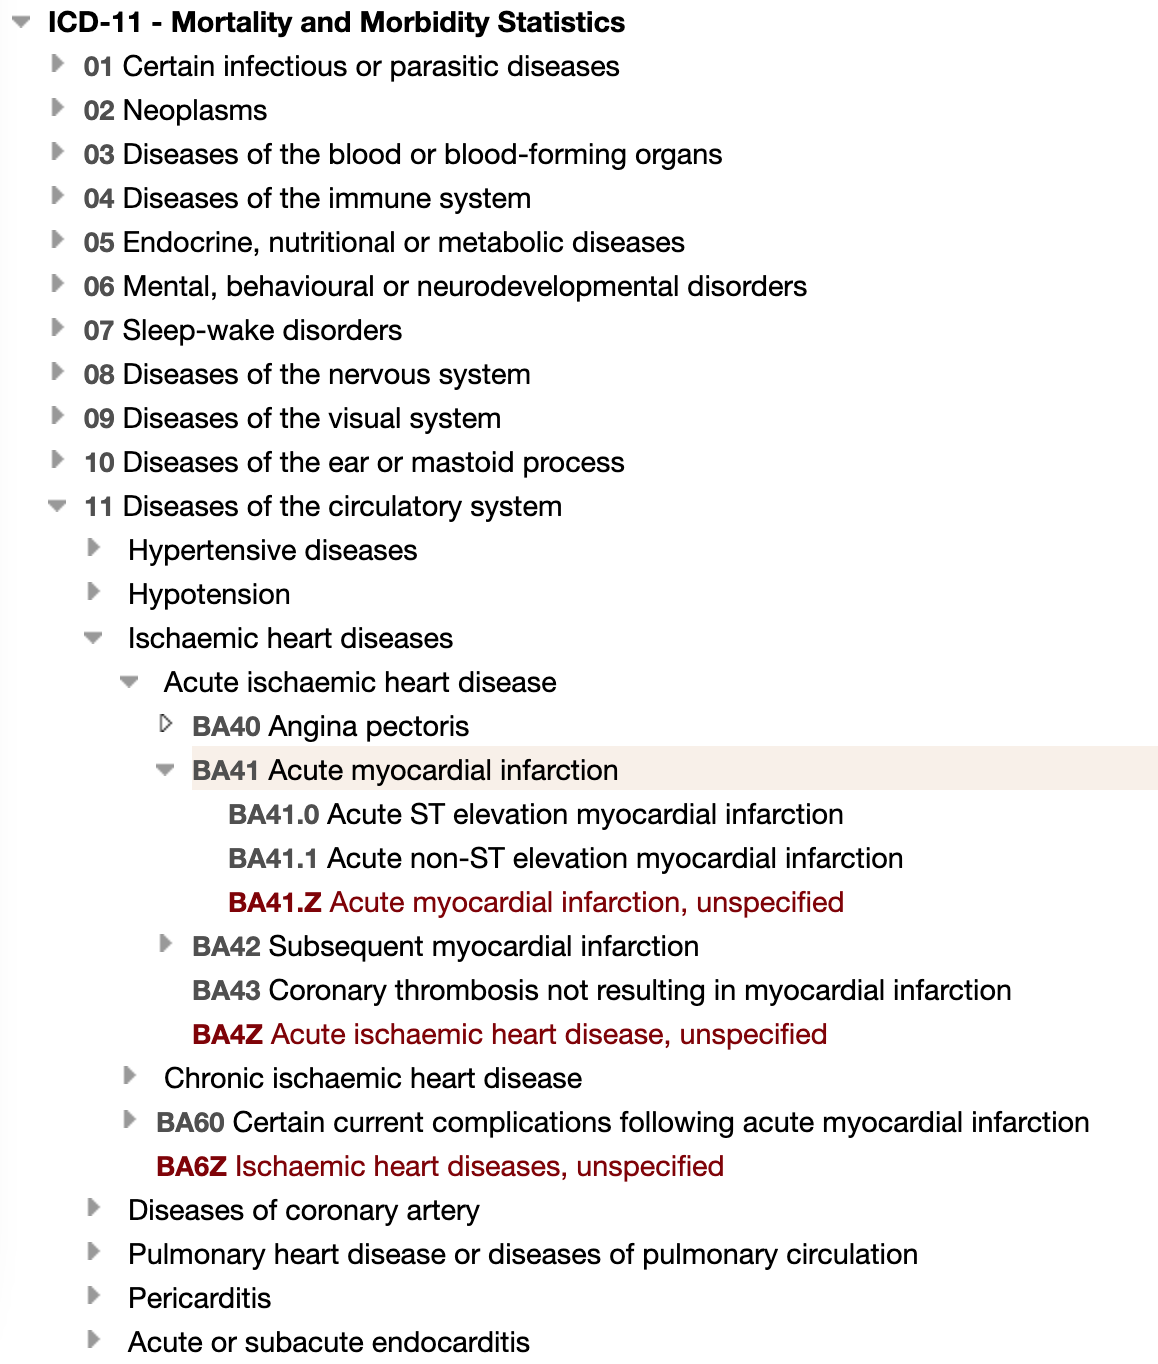
\includegraphics[width=0.8\textwidth]{icu_icd_mi}
\caption{ICD Codes}
\vspace{12px}
The International Classification of Diseases (ICD) is a taxonomy of all medical conditions maintained by the World Health Organization.  ``Acute myocardial infarction", for example, is a descendant of ``Acute ischemic heart diseases", which itself is a descendant of ``Ischemic heart diseases", which itself is a descendant of ``Diseases of the circulatory system".  ``Acute myocardial infarction" is then further subdivided if more granularity is required.
\label{fig:icu_icd_mi}
\end{figure}
    
\begin{figure}
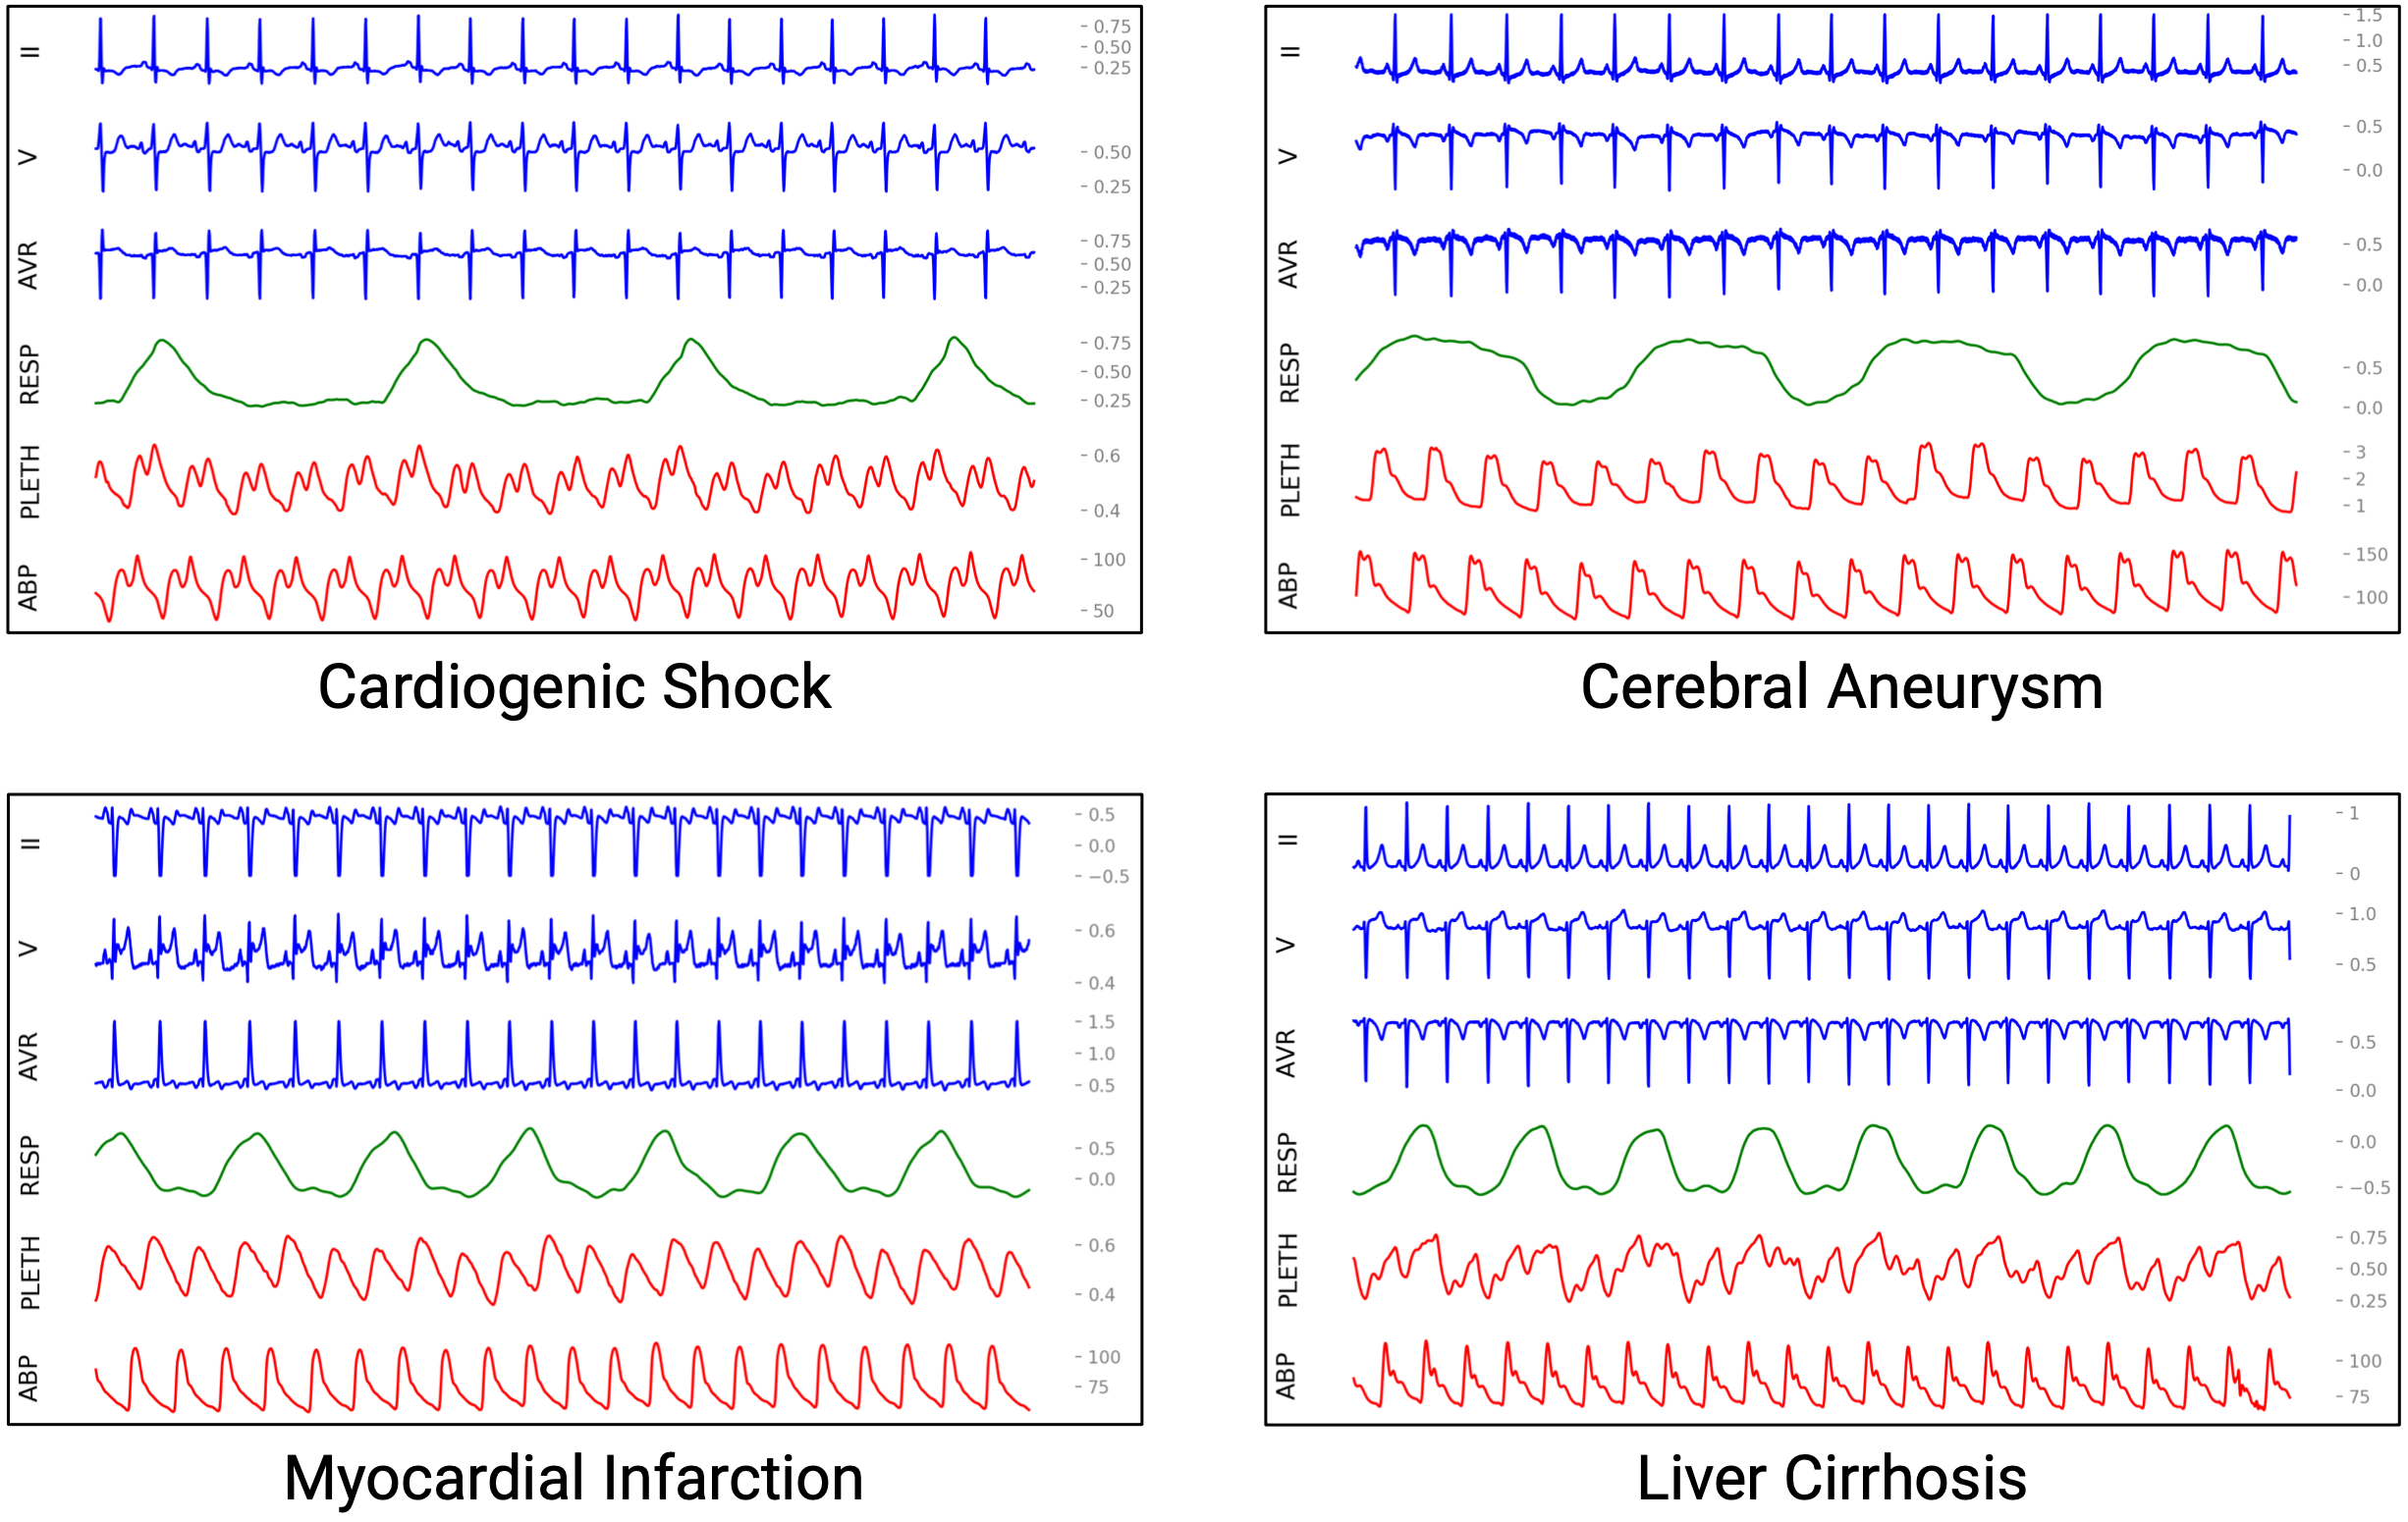
\includegraphics[width=\textwidth]{icu_example_inputs}
\caption{Example inputs}
\vspace{12px}
Waveforms are sampled at 125Hz with 8 bit resolution.  An example contains 2048 samples, or about 16 seconds.  Waveform types include 3 ECG leads (II, V, AVR) shown in blue, respiration shown in in green, and photoplethysmogram and arterial blood pressure, both shown in red.  An example is labeled with a set of ICD codes.  The examples shown were correctly detected by the net.  That is, the patient that produced the waveforms shown was eventually diagnosed with the ICD code below.  In the upper left we see an example from a patient that was correctly flagged for cardiogenic shock.  The the upper right we have an example of a detected cerebral aneurysm.  In the lower left and right we have examples of myocardial infarction and liver cirrhosis.
\label{fig:icu_example_waveforms}
\end{figure}

Consider a clean dataset $\mathcal{D}$ of waveforms $x$ and ICD codes $y$.  The dataset contains $n > 10,000$ patients and each patient $i$ had a hospital stay long enough to produce $m_i$ examples.  Each example contains $|\mathcal{S}|=15$ waveforms sampled at 125Hz for $T = 2048$ samples, or about 16 seconds.  If a patient did not have waveform $s$ measured for example $j$, then $x_{ijs} = \mathbf{0} \in \mathbb{R}^T$.  The label $y_i$ for patient $i$ is a vector of $d=90$ binary values and $y_{ik} = 1$ if patient $i$ was diagnosed for ICD code $k$.  The dataset is described as follows
\begin{gather}
    \mathcal{D} = \{
        (x_{ij}, y_i),
        \text{ for } i \in \{ 1, \dots, n \},
        \text{ for } j \in \{ 1, \dots, m_i \}
    \} \\
    x_{ij} \in \mathcal{X} = \mathbb{R}^{|\mathcal{S}| \times T} \\
    y_i \in \mathcal{Y} = \{0, 1\}^d
\end{gather}

Consider a neural net $f$ that takes as input an example $x$ comprised of $k=15$ different waveforms, each with $T=2048$ samples.  The net is also given parameters $\theta \in \Theta$.  The net used contained $|\Theta| = 6,721,114$ parameters.  The net outputs a vector of binary outcome probabilities $p$, one probability for each of the $d=90$ ICD codes.
\begin{gather}
    f: \mathcal{X} \times \Theta \mapsto \mathcal{P} = [0, 1]^d \\
    p = f(x, \theta)
\end{gather}
When the net makes a prediction, it is penalized by a loss function $\ell$.  The loss function takes as input the vector of probabilities $p$ that the net predicted, along with the vector of actual ICD code diagnoses $y$.  For each ICD code $k$ the binary cross entropy is computed between the prediction $p_k$ and and label $y_k$.  The loss is then the average binary cross entropy over all $d=90$ ICD codes.
\begin{gather}
    \ell: \mathcal{P} \times \mathcal{Y} \mapsto \mathbb{R} \\
    \ell(p, y) = -\frac{1}{d} \sum_{k=1}^d 
        y_k * \log p_k + (1 - y_k) * \log(1 - p_k)
\end{gather}
The net is trained with batches of examples of size $b = 32$.  The batch loss $L$ is the sum of individual losses $\ell$.
\begin{align}
    L &: \mathcal{X}^b \times \mathcal{Y}^b 
        \times \Theta \mapsto \mathbb{R}, \quad
        X \in \mathcal{X}^b, \quad 
        Y \in \mathcal{Y}^b \\
    L(X, Y, \theta) 
        &= \sum_{i=1}^b \ell(f(x_i, \theta), y_i) \\
        &= \sum_{i=1}^b \ell(p_i, y_i) \\
        &= -\frac{1}{d} \sum_{i=1}^b \sum_{k=1}^d 
            y_{ik} * \log p_{ik} + (1 - y_{ik}) * \log(1 - p_{ik})
\end{align}
The parameters $\theta$ are computed with stochastic gradient descent.  The batch loss $L$ is differentiable with respect to the $j$th parameter of $\theta$.
\begin{align}
    \frac{\partial L}{\partial \theta_j} 
        &= \sum_{i=1}^b \sum_{k=1}^d 
            \frac{\partial \ell}{\partial p_{ik}}  
            \frac{\partial p_{ik}}{\partial \theta_j} \\
        &= \frac{1}{d} \sum_{i=1}^b \sum_{k=1}^d
            \left(
                \frac{1 - y_{ik}}{1 - p_{ik}} - \frac{y_{ik}}{p_{ik}}
            \right)
            \frac{\partial p_{ik}}{\partial \theta_j}
\end{align}
To complete this batch loss derivative, and perform gradient descent to compute the parameters $\theta$, the net $f$ must be differentiable with respect to its parameters $\theta$.

\subsection{Model Architecture}

To take advantage of the stationary nature of the waveforms, a 1D ConvNet was used.  If the waveforms were properly aligned, it would make sense to have convolution kernels span all the waveforms at once and convolve along the time dimension.  The waveforms, however, are not properly aligned.  They are misaligned by up to 500 ms, or about 64 samples.  This is on the order of the entire size of a convolution kernel.  In fact, the largest convolution kernels in the entire net were only 16 samples long.  To deal with the misalignment, the first 4 layers of the net convolve along the waveforms independently.  After 4 layers, each activation has a larger receptive field.  Dilated convolutions were used to help with this.  Stacked dilated convolutions enable networks to have very large receptive fields with just a few layers, while preserving the input resolution throughout the network \cite{oord2016wavenet}.  

Residual layers are used to train a deep network and avoid vanishing gradients \cite{he2016deep}.  These networks were originally developed for computer vision applications but can be used here as well.  To compute the activations $z$ in layer $\ell + 1$ from the activations in layer $\ell$, a residual layer takes the form
\begin{gather}
    z^{(\ell + 1)} = f(z^{(\ell)}) + z^{(\ell)}
\end{gather}
These skip connections allow data and gradients to flow unimpeded by the layers, allowing for deeper networks to be trained more aggressively.

The first 4 layers of the net are 1D dilated independent convolutions with skip connections.  The remaining 8 layers are 1D dilated joint convolutions with skip connections.  Finally there is a dense layer at the end.  The biases of the final layer are initialized such that the network predicts the prior of that condition when first initialized.  That is, if the prevalence of ICD code $k$ is $\pi_k$, then the $k$th bias is set to the inverse sigmoid of $\pi_k$
\begin{gather}
    \text{bias}_k = \log \pi_k - \log(1 - \pi_k)
\end{gather}
Predicting the prevalence minimizes the binary cross entropy if only the prevalence is known.

\subsection{Partition}

Valid patient indices $\mathcal{I}$ are partitioned randomly into 3 sets, ($\mathcal{I}_1$, $\mathcal{I}_2$, $\mathcal{I}_3$), to be used for 3-fold cross-validation.  Patient $i$ is a valid test patient if the set of signals recorded for their stay $\mathcal{S}_i$ contains all the required waveforms specified by the set $\mathcal{S}_{test}$
\begin{gather}
    \mathcal{S}_{test} = \{ \text{PLETH, ABP, RESP, II, V, AVR} \}
\end{gather}
This set of required waveforms was chosen because they were commonly measured in the dataset.  The 3-fold partition of test patients is then
\begin{align}
    \mathcal{I} 
        &= \{
            i \in \{1, \dots, n\} \mid 
            \mathcal{S}_{test} \subseteq \mathcal{S}_i
        \} \\
        &= \mathcal{I}_1 \cup \mathcal{I}_2 \cup \mathcal{I}_3 \text{ where }
            \mathcal{I}_1 \cap \mathcal{I}_2 = \emptyset, \mathcal{I}_1 \cap \mathcal{I}_3 = \emptyset
\end{align}
Each fold defines a training dataset $\mathcal{D}_{train}$ and a testing dataset $\mathcal{D}_{test}$.  A patient that does not have all of the required waveforms measured for testing is still used for training with the missing waveforms represented with 0s.  The net was trained until the training loss started to plateau.  In prior experiments, this was fairly consistent with when the validation loss started to increase, i.e. the net was overfitting. The training and testing datasets are defined as
\begin{gather}
    \mathcal{D}_{test} = \{
        (x_{ij}, y_i),
        \text{ for } i \in \mathcal{I}_k,
        \text{ for } j \in \{ 1, \dots, m_i \}
    \} \\
    \mathcal{D}_{train} = \{
        (x_{ij}, y_i),
        \text{ for } i \in \{1, \dots, n\} - \mathcal{I}_k,
        \text{ for } j \in \{ 1, \dots, m_i \}
    \}
\end{gather}
When training and testing, each patient should carry equal weight.  Since each patient was in the hospital for different lengths of time, it is easy to bias the distribution of training and testing data toward patients who are in the hospital for longer periods of time.  To remove this bias, a simple procedure is used.  When training or testing, first randomly sample a patient, and then randomly sample a segment from their hospital stay.
\begin{gather}
    i \sim \text{uniform}(\mathcal{I}) \\
    j \sim \text{uniform}(\{1, \dots, m_i\})
\end{gather}
The per-patient example count $m_i$ can then be replaced by a constant $m$, since the same number of examples is drawn for each patient.
\begin{gather}
    \mathcal{D} = \{
        (x_{ij}, y_i),
        \text{ for } i \in \{ 1, \dots, n \},
        \text{ for } j \in \{ 1, \dots, m \}
    \}
\end{gather}

\begin{figure}
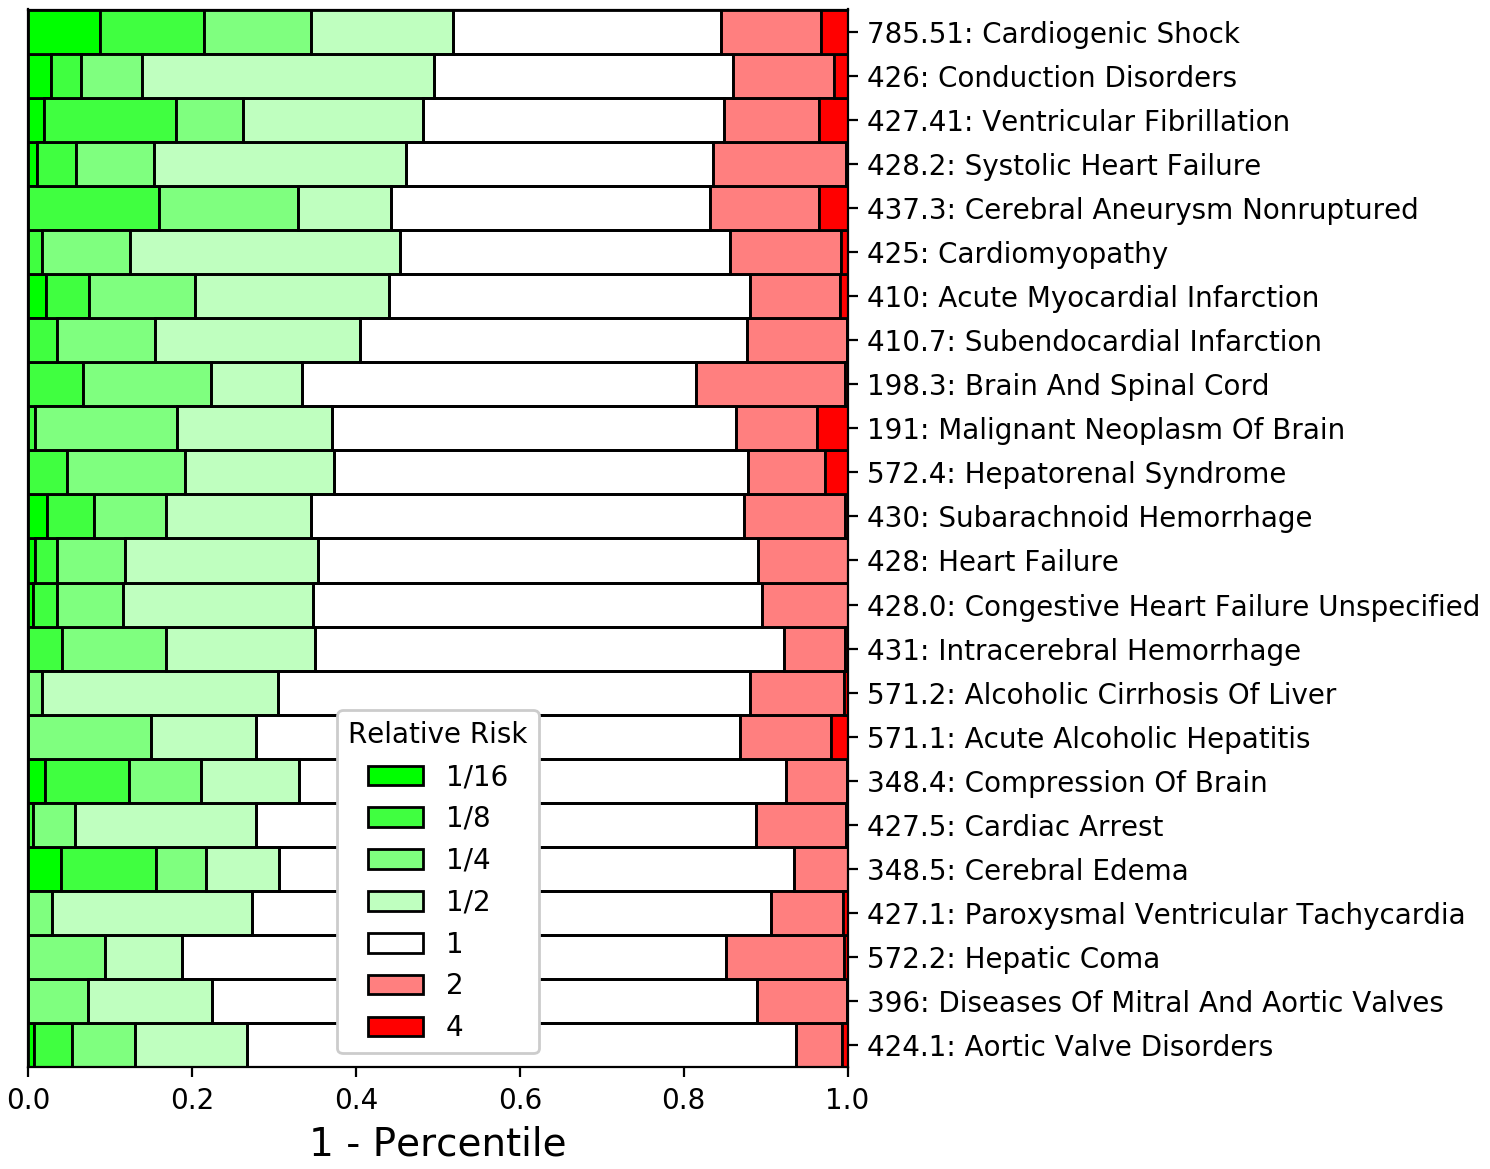
\includegraphics[width=\textwidth]{icu_relative_risk}
\caption{Relative risk}
\vspace{12px}
Patients are placed into estimated risk categories of powers of 2.  For example, a patient in the 1/4 risk category of systolic heart failure is estimated to be between 1/4 and 1/8 as likely to be diagnosed with systolic heart failure.  For cardiogenic shock, about half of the patients can be placed into a low risk category.  The risk level estimates are conservative, with low risk patients actually estimated to have lower risk than the risk group they are placed in, and high risk patients estimated to have higher risk than the risk group they are placed in.
\label{fig:icu_relative_risk}
\end{figure}

\begin{figure}
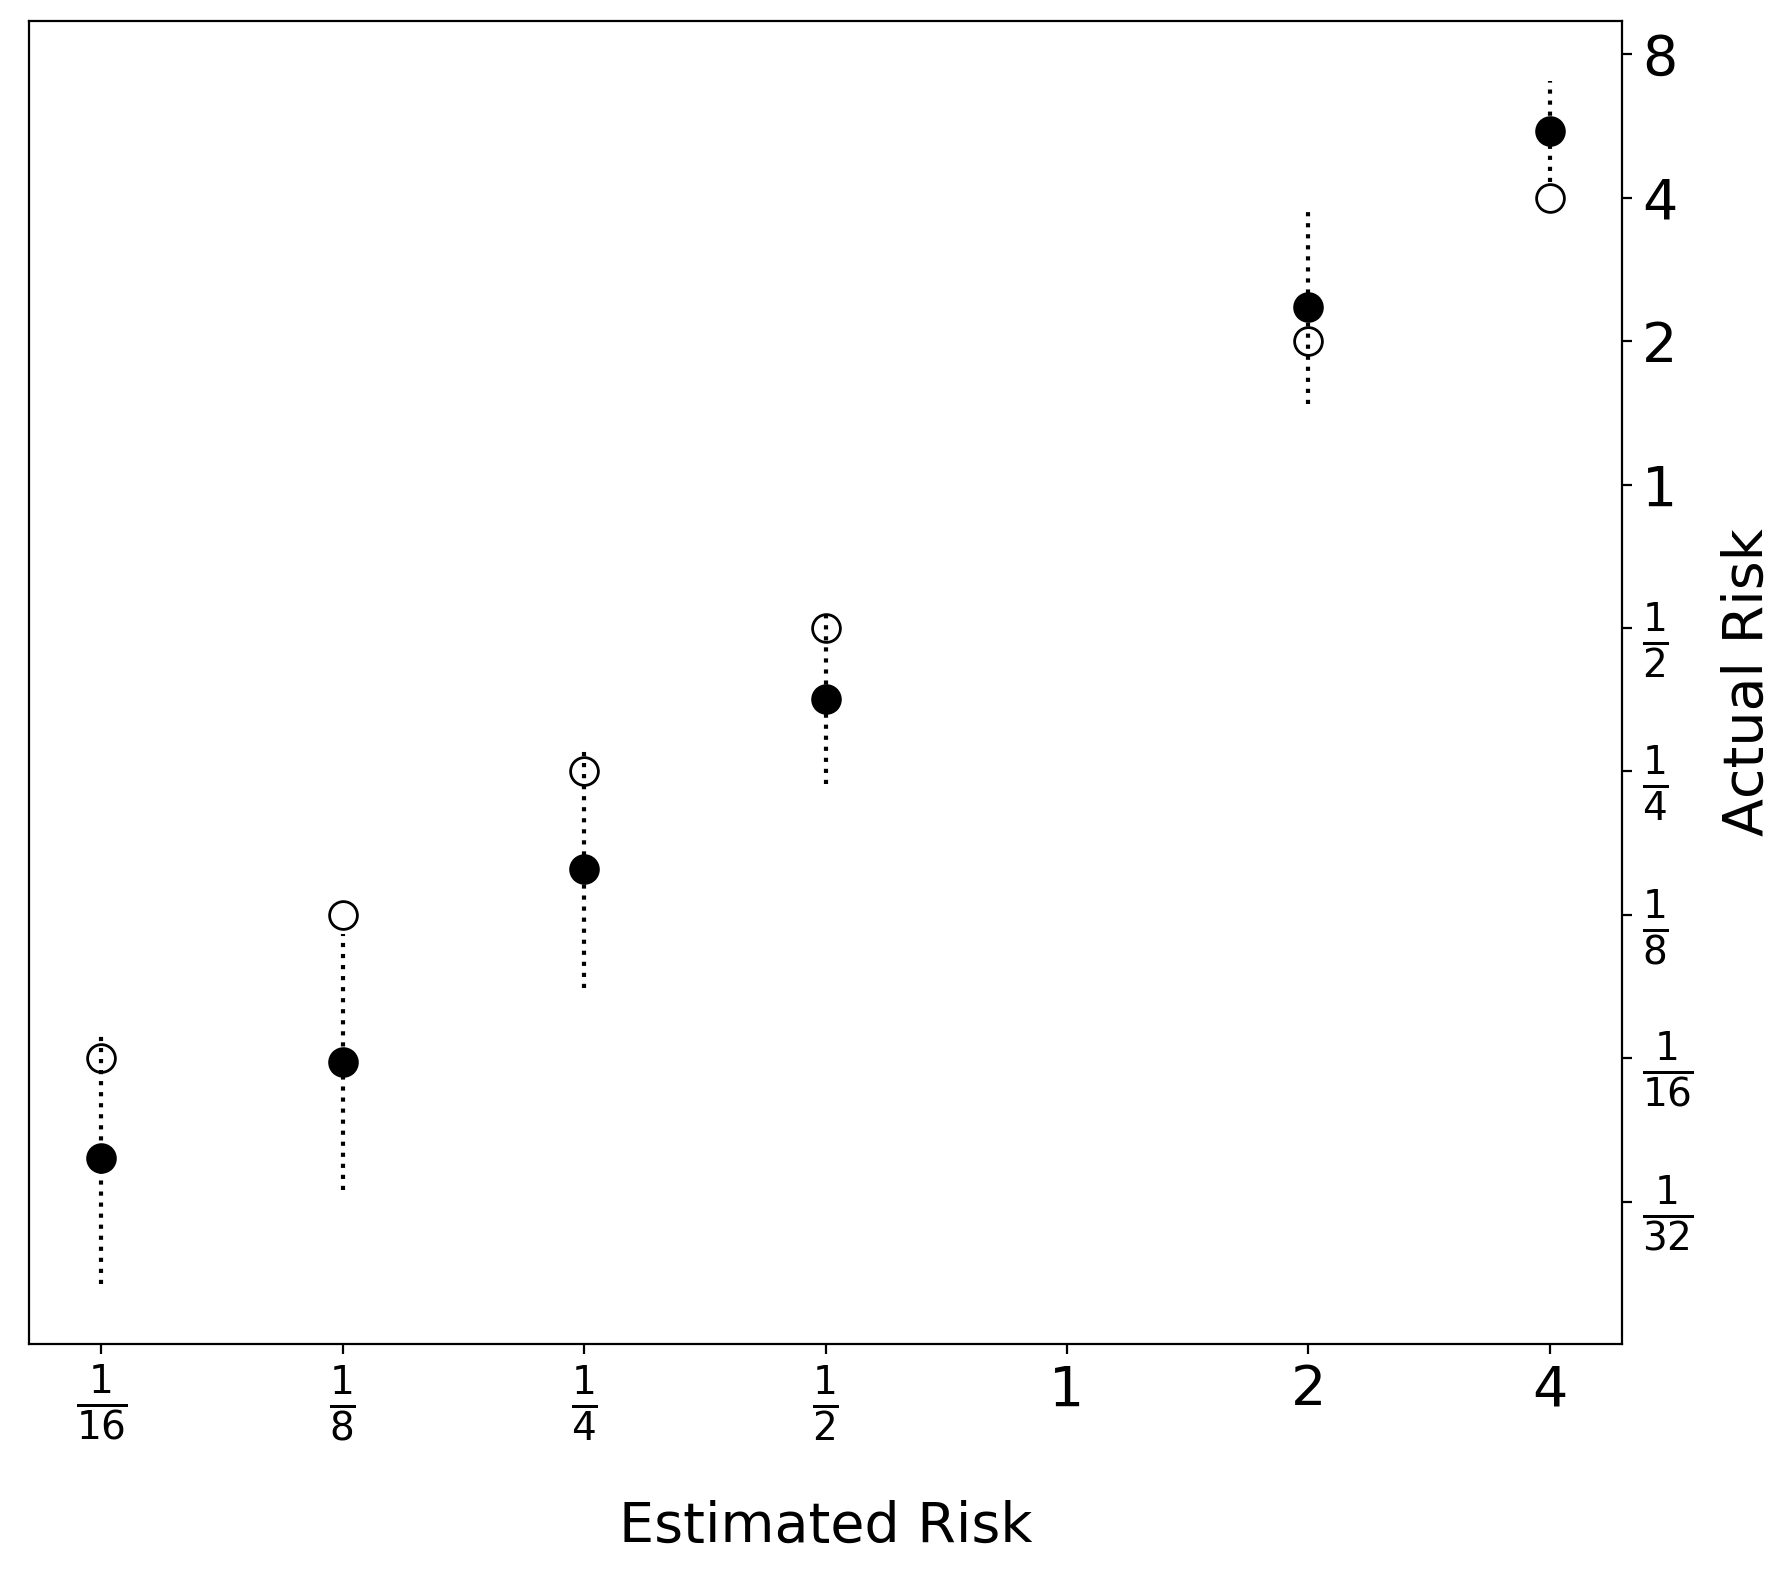
\includegraphics[width=\textwidth]{icu_actual_risk}
\caption{Actual risk}
\vspace{12px}
Risk categories are valid.  For each risk category an actual risk can be computed with error bars.  The error bars represent the fact that there are 90 conditions being predicted.  Ideally the low risk categories should have an actual risk lower than the estimated risk and the high risk categories should have a risk higher than the estimated risk, since the risk estimates were conservative.
\label{fig:icu_actual_risk}
\end{figure}

\pagebreak
\section{Results}

\subsection{Relative Risk}

After performing 3-fold cross validation, there is a prediction for every example in the test set.
\begin{gather}
    \mathcal{P} = \{
        p_{ij},
        \text{ for } i \in \mathcal{I},
        \text{ for } j \in \{ 1, \dots, m \}
    \}
\end{gather}
Just before the sigmoid in the final layer, there is an unnormalized representation of the net output, $p = \text{sigmoid}(z)$ where $z \in \mathbb{R}$ and $p \in [0, 1]$.
\begin{gather}
    \mathcal{Z} = \{
        z_{ij},
        \text{ for } i \in \mathcal{I},
        \text{ for } j \in \{ 1, \dots, m \}
    \}
\end{gather}
The empirical distributions over $z$ given $y$ can be used to compute a posterior.  Let $Y_k = 1 \mid Z_k = z$ be the event that a new patient is diagnosed with ICD code $k$ given that the net outputs value $z$ for that code.  Information on the reverse situation is known.  That is, there is information on the probability of the net outputting a value $z$ given that the patient is or is not diagnosed.  The prevalences of these conditions in the hospital are also known.  Let $\pi_k$ be the prevalence of ICD code $k$ among hospital patients.  Applying Bayes Rule:
\begin{gather}
    P(Y_k = 1 \mid Z_k = z) = \frac
        {P(Z_k = z \mid Y_k = 1) \ \pi_k}
        {P(Z_k = z \mid Y_k = 0) (1 - \pi_k) + P(Z_k = z \mid Y_k = 1) \ \pi_k}
\end{gather}
To naively estimate this posterior, one could compute 2 histograms of $Z_k \mid Y_k$, one each for $Y_k=0$ and $Y_k=1$.  That is, bin possible values of $Z_k$ and count how many times the net predicts a value within that range.  Do this for predictions when the label is negative for ICD code $k$, and again for predictions when the label is positive for ICD code $k$.  Finally one would normalize those histograms so that the total areas are 1.  If the bins are too small, the number of occurrences in a particular bin has high variance, and the empirical distribution will be far from smooth.  If the bins are too large, the empirical distribution will be very coarse.  Further, there is often very little data present for the situation when the label is positive for an ICD code.  Is there a more direct way, to avoid binning and counting?  Yes, there is Kernel Bayes Rule \cite{fukumizu2013kernel}.

Kernel Bayes Rule says that given a bunch of observations $(x_i, y_i)$ for $i = 1, \dots, n$, the posterior of $y$ given $x$ can be estimated using a positive definite kernel function $K$ as follows
\begin{gather}
    \hat{P}(Y = y | X = x) = \frac
        {\sum_{i=1}^n K(x - x_i) \ K(y - y_i)}
        {\sum_{i=1}^n K(x - x_i)}
\end{gather}
Applying Kernel Bayes Rule, the posterior can be directly estimated without discretizing and binning.
\begin{gather}
    \hat{P}(Y_k = 1 \mid Z_k = z) = \frac
        {\sum_{i \in \mathcal{I}} y_{ik} \sum_{j=1}^m K(z - z_{ijk})}
        {\sum_{i \in \mathcal{I}} \sum_{j=1}^m K(z - z_{ijk})}
\end{gather}
A standard radial basis function (RBF) kernel was used with $\sigma = 0.8$.  For examples of these kernel densities, see Figures \ref{fig:icu_cardio}, \ref{fig:icu_systolic}, \ref{fig:icu_cerebral}, \ref{fig:icu_myocard}.

When computing this posterior, it is important that no prediction should depend on its label.  Consider the following naive posterior calculation for a test patient $i$
\begin{gather}
    \hat{P}(Y_{ik} = 1 \mid Z_k = z_{ijk}) = \frac
        {\sum_{i' \in \mathcal{I}} y_{i'k} \sum_{j'=1}^m K(z_{ijk} - z_{i'j'k})}
        {\sum_{i' \in \mathcal{I}} \sum_{j'=1}^m K(z_{ijk} - z_{i'j'k})}
\end{gather}
There are two issues here.  First, the summation over test patients $\mathcal{I}$ must not include the test patient of interest $i$, otherwise $y_{ik}$ is being used to predict the outcome $Y_{ik}$.  Second, remember that the net output is a function of its parameters, $z_{ij} = f(x_{ij}, \theta)$, and the parameters $\theta$ are a function of the training dataset $\mathcal{D}_{train}$ via gradient descent.  It follows then that to compute a posterior without using its label, the summation must be over all patients in the test set except for the patient of interest $\mathcal{I}_{test} - i$.
\begin{gather}
    \hat{P}(Y_{ik} = 1 \mid Z_k = z_{ijk}) = \frac
        {\sum_{i' \in \mathcal{I}_{test} - i} y_{i'k} \sum_{j'=1}^m K(z_{ijk} - z_{i'j'k})}
        {\sum_{i' \in \mathcal{I}_{test} - i} \sum_{j'=1}^m K(z_{ijk} - z_{i'j'k})}
\end{gather}
The relative risk $r$ can be computed for every patient $i$ in the test set, for every example from their stay $j$, and for every ICD code $k$.
\begin{gather}
    r_{ijk} = \frac
        {\hat{P}(Y_{ik} = 1 \mid Z_k = z_{ijk})}
        {\pi_k}
\end{gather}
Given relative risk bounds $(r_{\min}, r_{\max})$ examples can be placed into relative risk groups $\mathcal{G}_k$ for each condition $k$
\begin{gather}
    \mathcal{G}_k(r_{\min}, r_{\max}) = \{ (i, j) \mid r_{\min} < r_{ijk} < r_{\max} \}
\end{gather}
This grouping serves to later assess the validity of the relative risk predictions across ICD codes.  The relative risks are grouped by powers of 2.  For example, for the ICD code of cardiogenic shock and relative risk group bounded by $r_{\min} = 2$, $r_{\max} = 4$ represents patients flagged to carry twice the estimated risk for experiencing a cardiogenic shock sometime during their hospital stay.  The estimated 2x risk for that group is a conservative estimate since patients in that group could carry as much as 4x the risk.  Similarly, the relative risk group bounded by $r_{\min} = 1/4$, $r_{\max} = 1/2$ represents patients flagged to carry half the estimated risk for experiencing cardiogenic shock sometime during their hospital stay.  Here, the conservative estimate of 1/2 for the low risk group corresponds to $r_{\max}$ rather than $r_{\min}$ as with the high risk group.  A grouping of all patients into risk groups for 24 conditions is shown in Figure \ref{fig:icu_relative_risk}.

Are the risk groups correct?  For each risk group $g = (r_{\min}, r_{\max})$ and ICD code $k$, the actual risk $a_k(g)$ observed can be computed.  It is computed as the fraction of examples that fall within that risk group that were ultimately diagnosed with ICD code $k$, divided by the prevalence of that condition $\pi_k$.
\begin{gather}
    a_k(g) = \frac{1}{\pi_k} \left( 
        \frac{\sum_{(i, j) \in \mathcal{G}_k(g)} y_{ik}}{|\mathcal{G}_k(g)|}
    \right)
\end{gather}
The means and standard deviations of actual risk for each risk group can be computed
\begin{gather}
    \mu(g) = \frac{1}{d} \sum_{k=1}^d a_k(g) \\
    \sigma^2(g) = \frac{1}{d} \sum_{k=1}^d (a_k(g) - \mu(g))^2
\end{gather}
These are plotted in Figure \ref{fig:icu_actual_risk}.  The results show that the observed risk for each group is in fact better than the conservative estimate, for all groups.  That is, for low risk groups, the observed risk is lower and for high risk groups, the observed risk is higher.

\begin{figure}
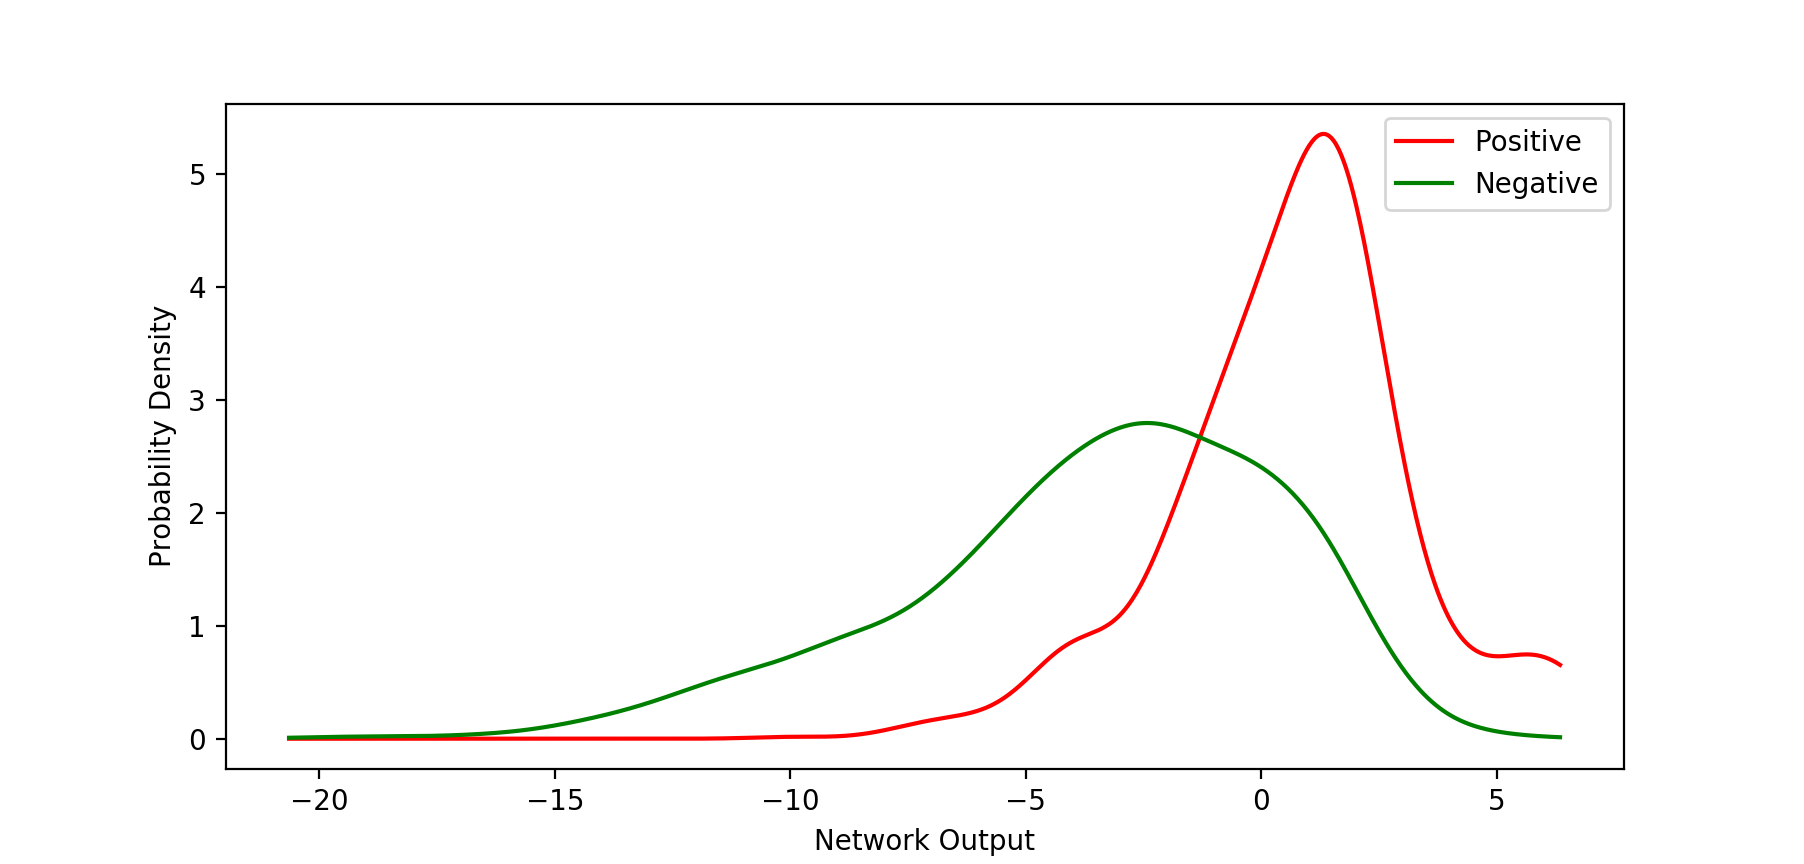
\includegraphics[width=\textwidth]{icu_cardio_prob}
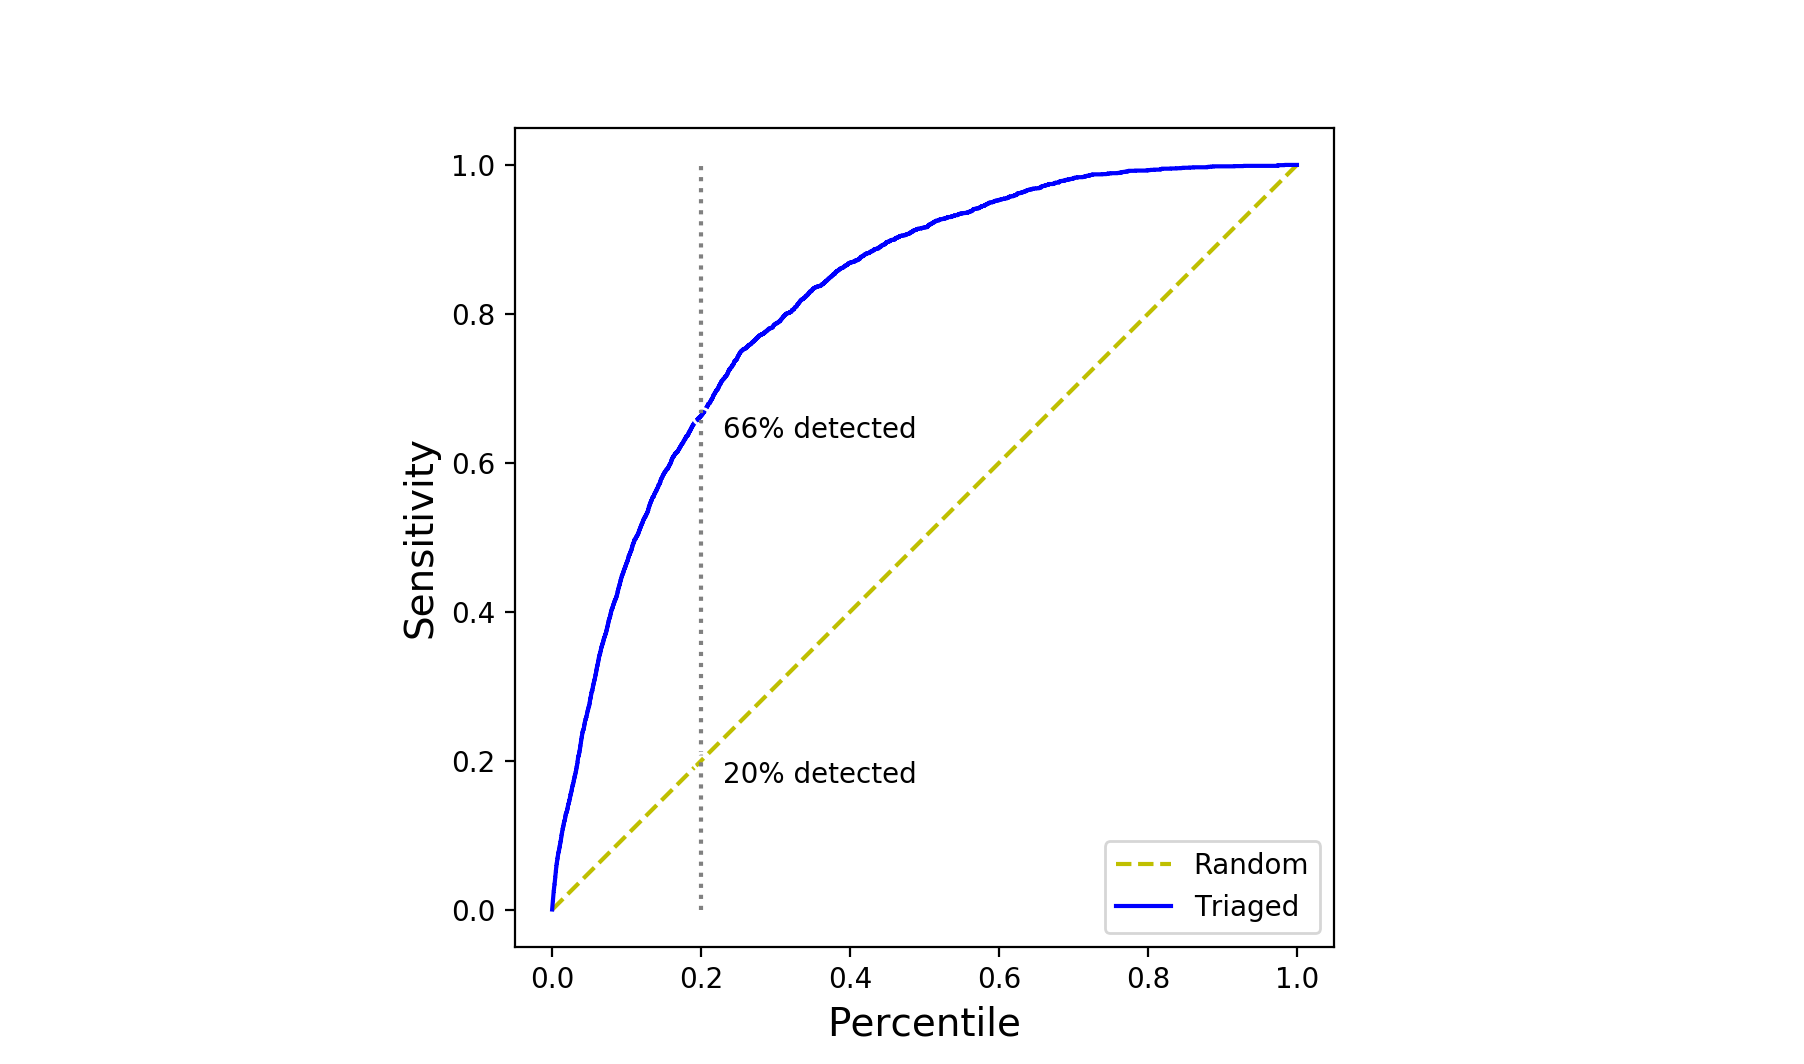
\includegraphics[width=\textwidth]{icu_cardio_sens}
\caption{Cardiogenic Shock Results}
\vspace{12px}
(a) Kernel density estimates of the net's output given whether the patient eventually receives a positive or negative diagnosis for cardiogenic shock. (b) Effective sensitivity of the network for detecting a cardiogenic shock.  Using the net to flag the 20 percentile patients at highest risk for further testing would detect 66\% of the cases.
\label{fig:icu_cardio}
\end{figure}

\begin{figure}
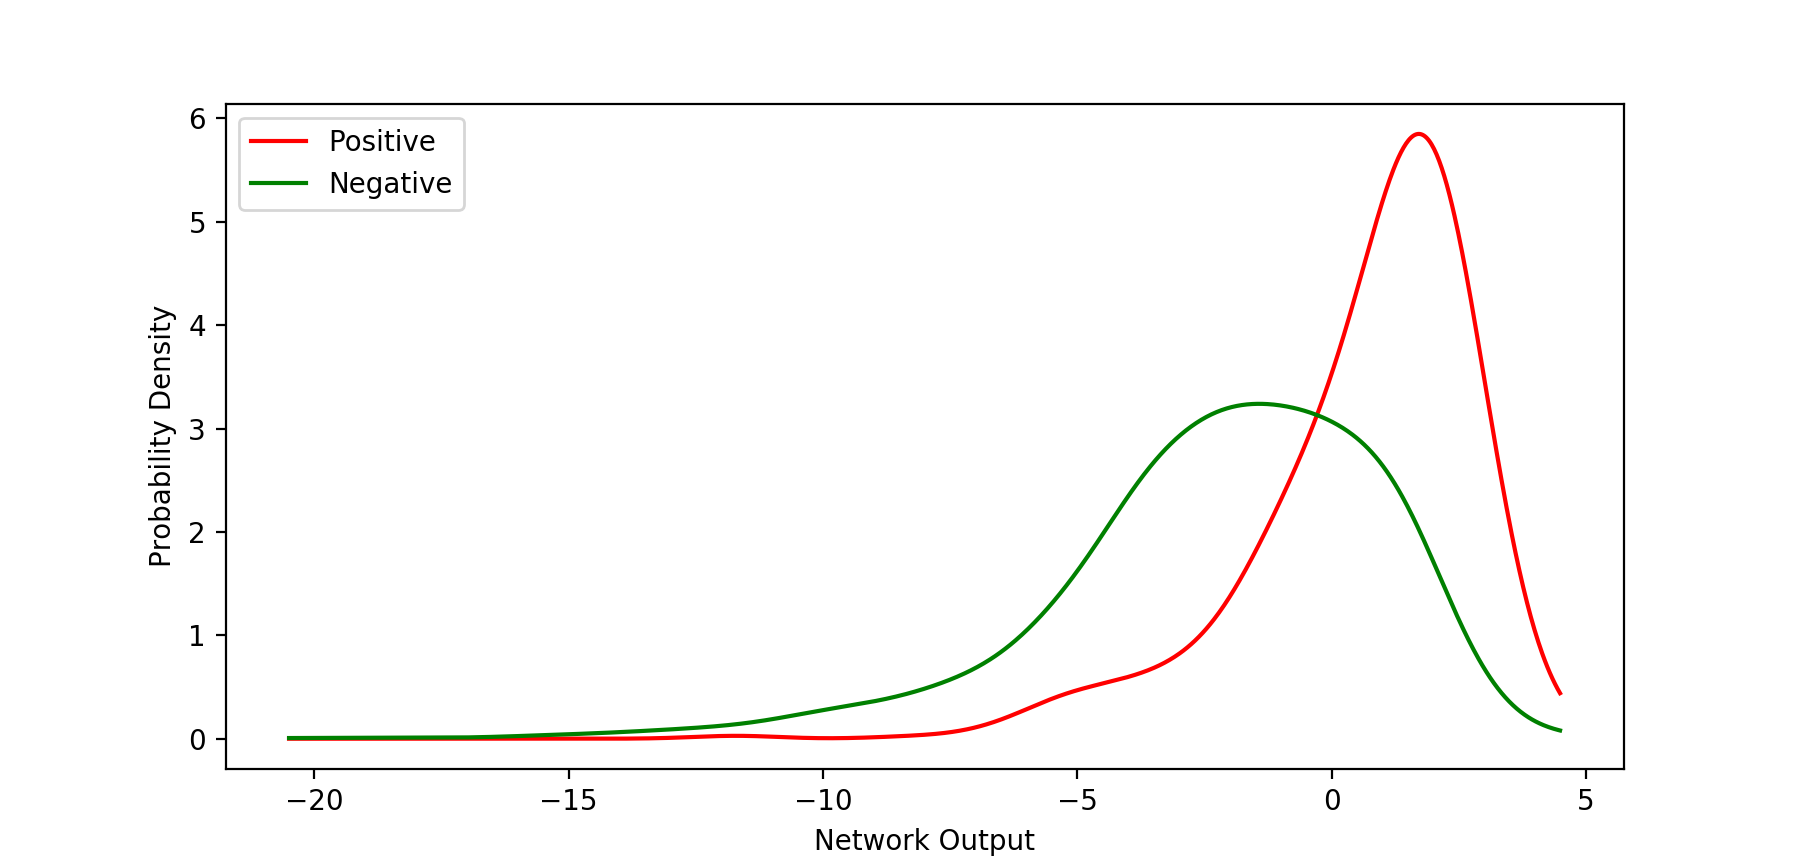
\includegraphics[width=\textwidth]{icu_systolic_prob}
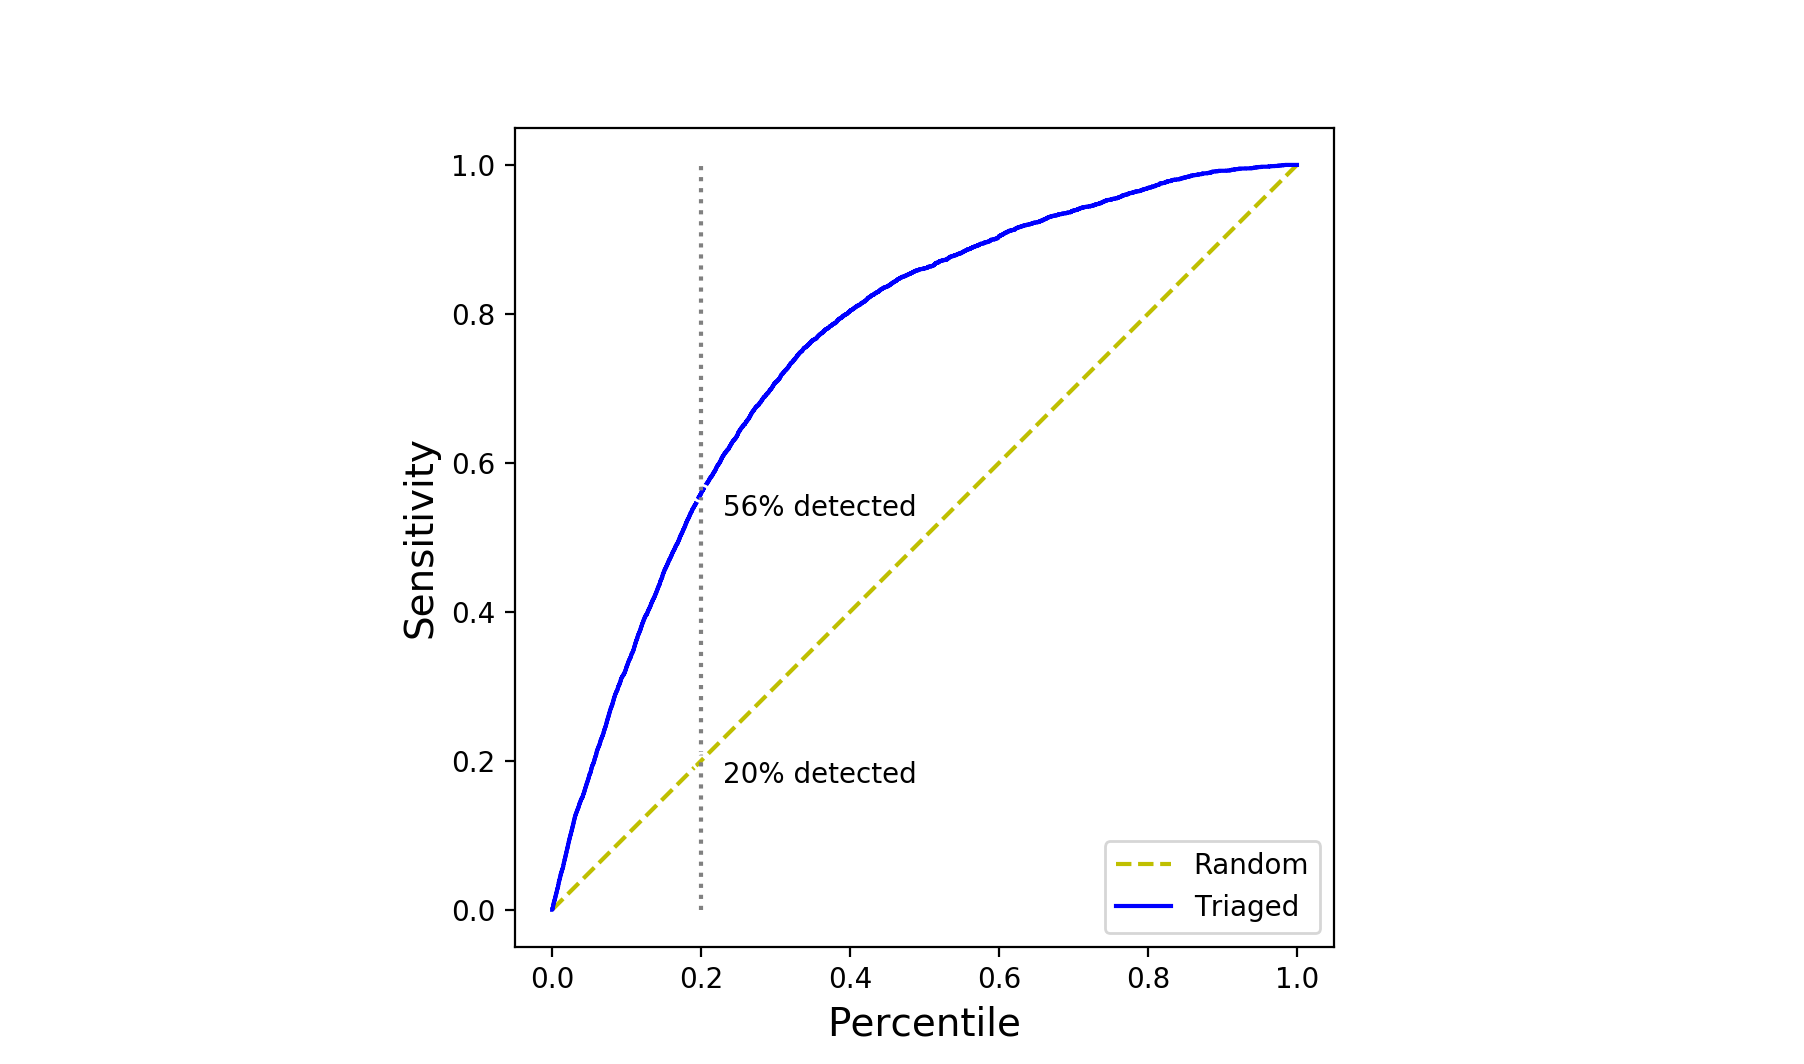
\includegraphics[width=\textwidth]{icu_systolic_sens}
\caption{Systolic Heart Failure Results}
\vspace{12px}
(a) Kernel density estimates of the net's output given whether the patient eventually receives a positive or negative diagnosis for systolic heart failure. (b) Effective sensitivity of the network for detecting systolic heart failure.  Using the net to flag the 20 percentile patients at highest risk for further testing would detect 56\% of the cases.
\label{fig:icu_systolic}
\end{figure}

\begin{figure}
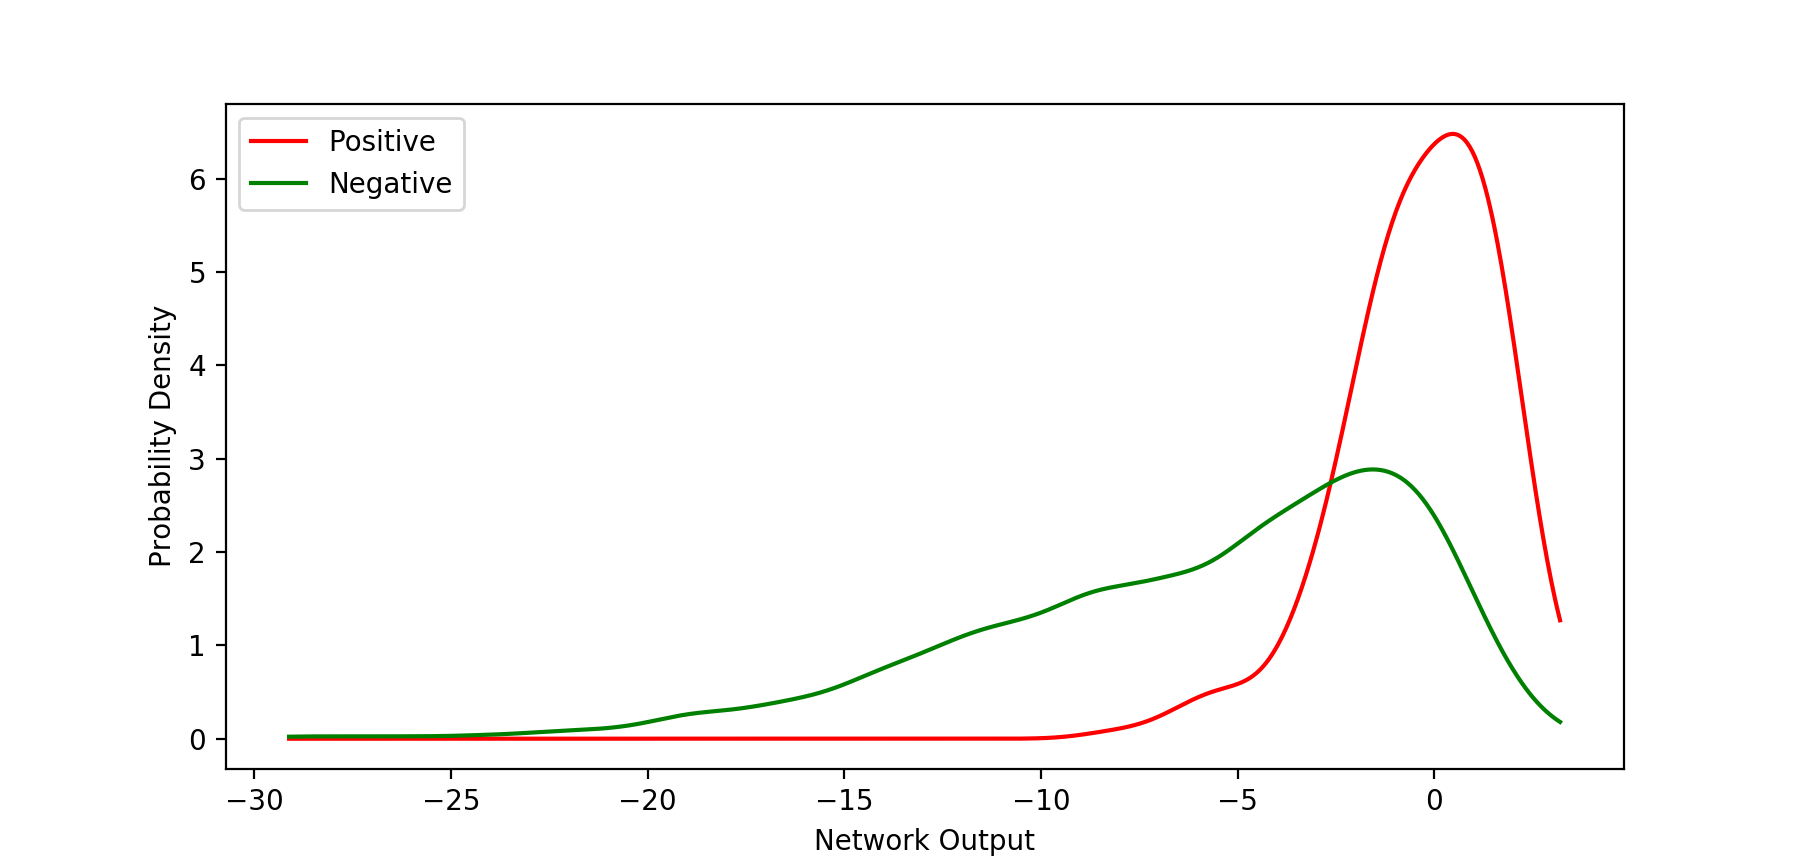
\includegraphics[width=\textwidth]{icu_cerebral_prob}
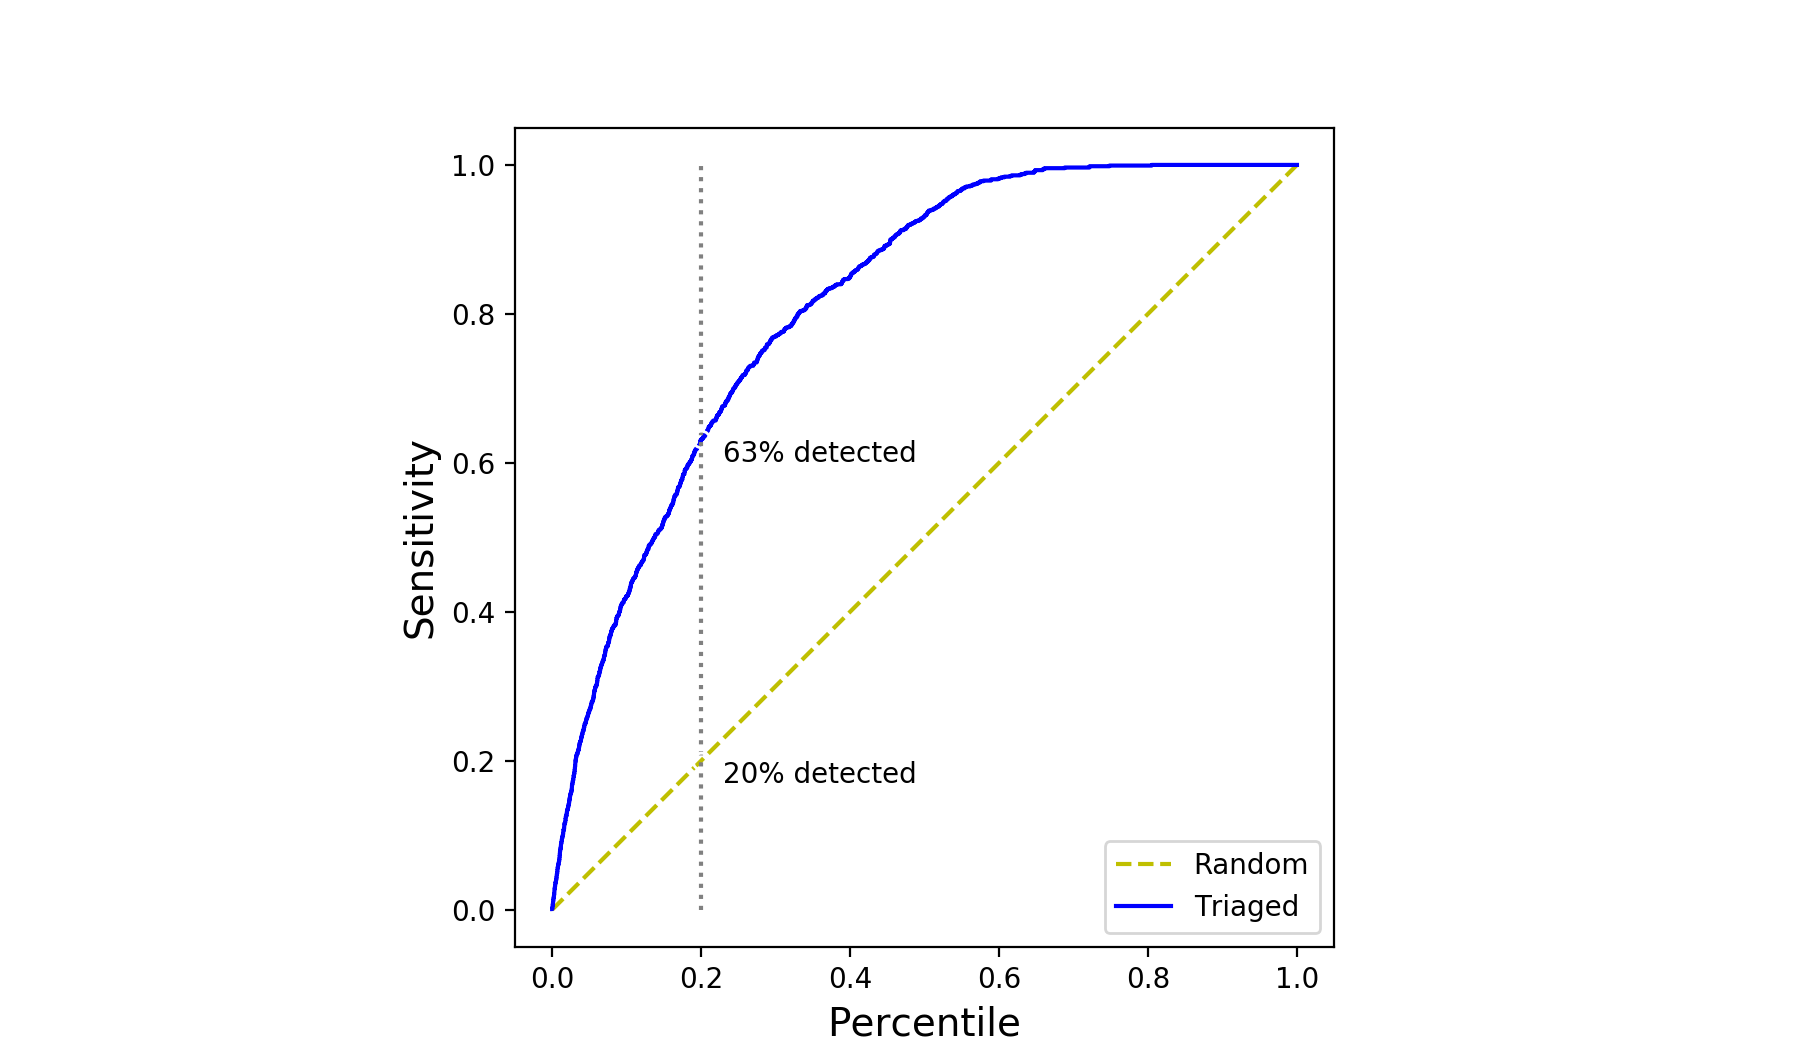
\includegraphics[width=\textwidth]{icu_cerebral_sens}
\caption{Cerebral Aneurysm Results}
\vspace{12px}
(a) Kernel density estimates of the net's output given whether the patient eventually receives a positive or negative diagnosis a cerebral aneurysm. (b) Effective sensitivity of the network for detecting a cerebral aneurysm.  Using the net to flag the 20 percentile patients at highest risk for further testing would detect 63\% of the cases.
\label{fig:icu_cerebral}
\end{figure}
    
\begin{figure}
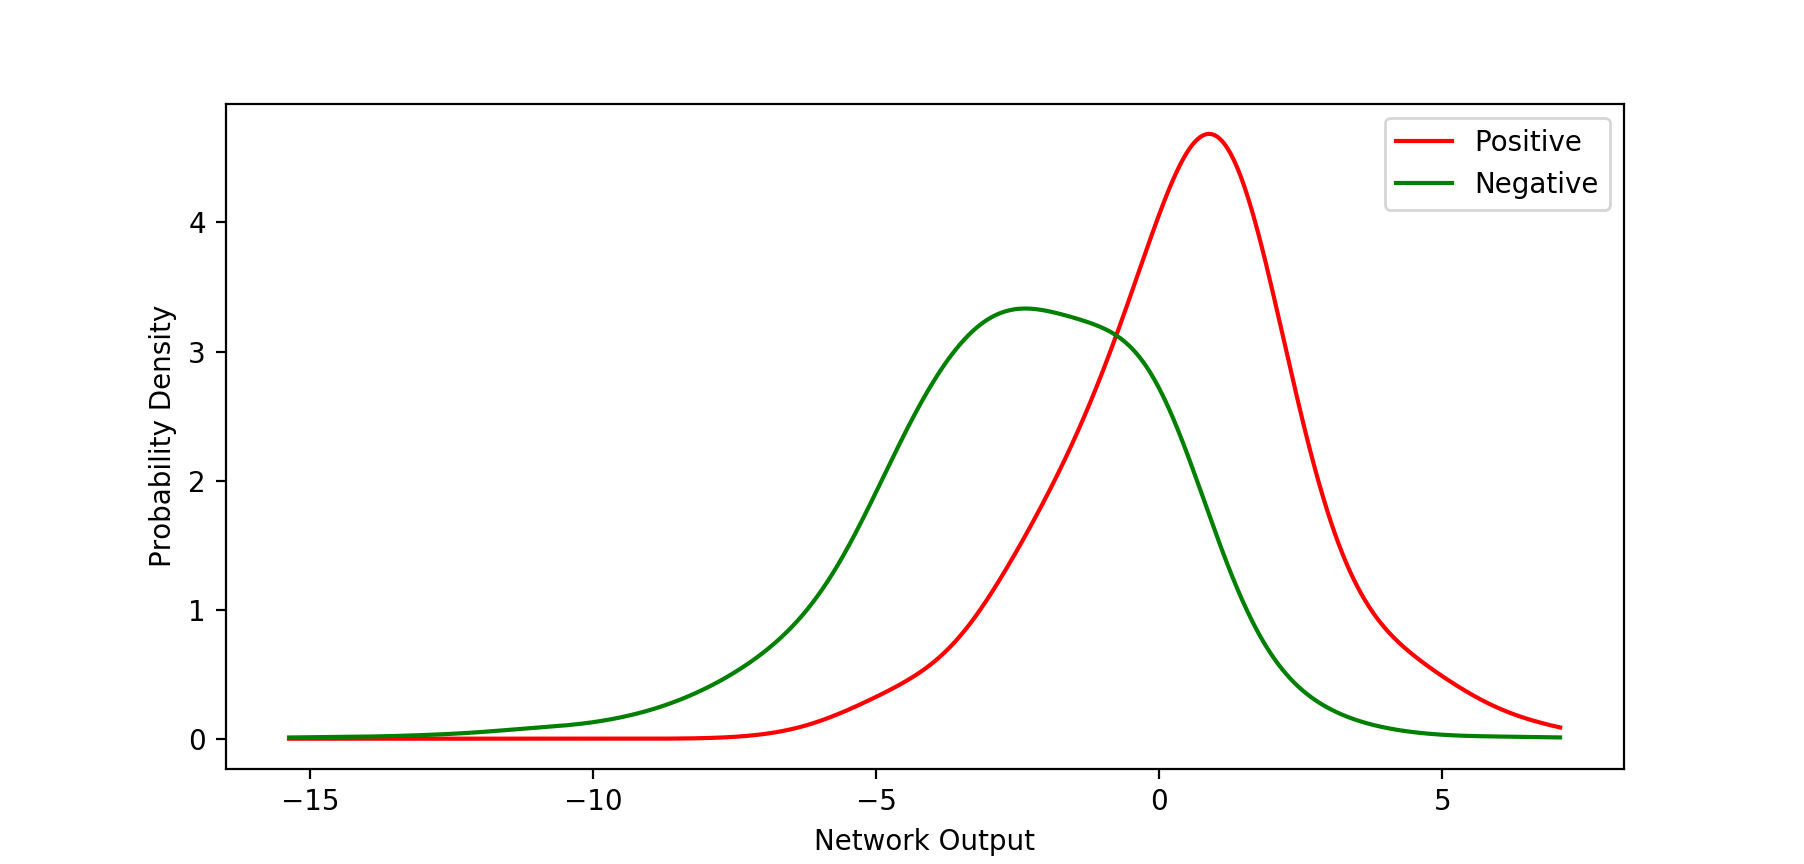
\includegraphics[width=\textwidth]{icu_myocard_prob}
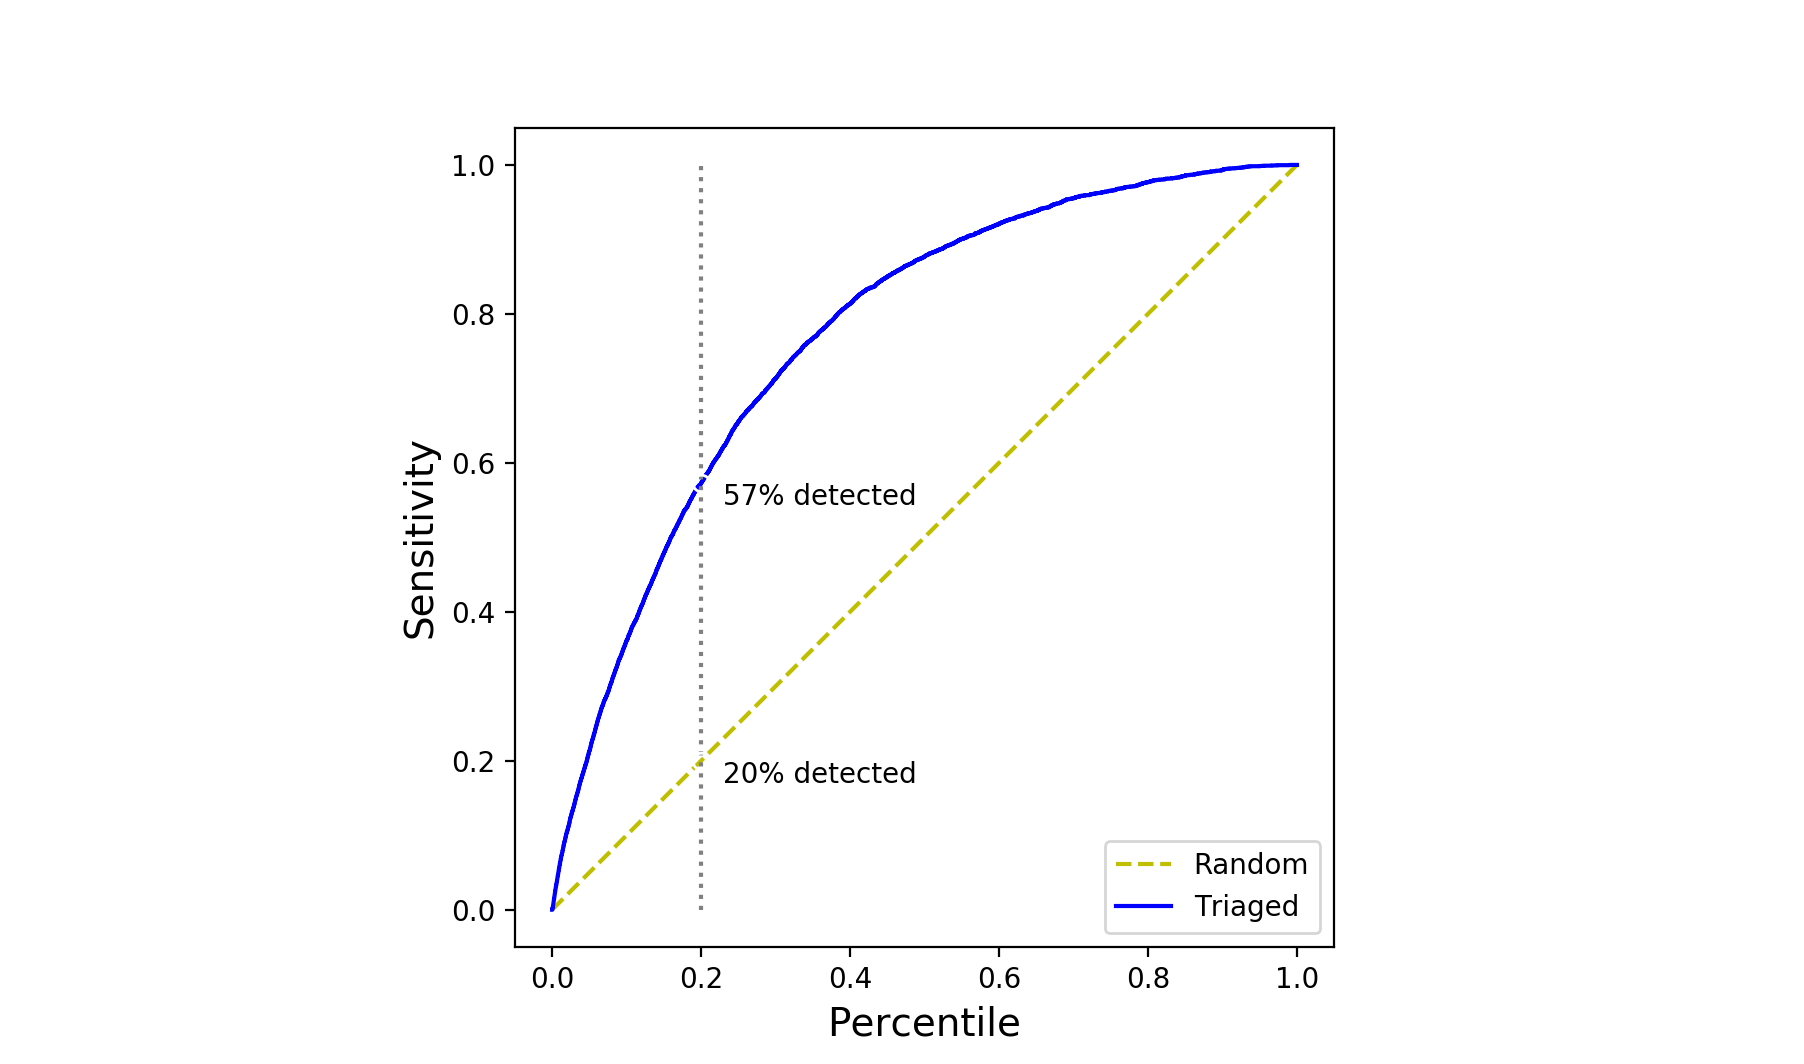
\includegraphics[width=\textwidth]{icu_myocard_sens}
\caption{Myocardial Infarction Results}
\vspace{12px}
(a) Kernel density estimates of the net's output given whether the patient eventually receives a positive or negative diagnosis for myocardial infarction. (b) Effective sensitivity of the network for detecting a myocardial infarction.  Using the net to flag the 20 percentile patients at highest risk for further testing would detect 57\% of the cases.
\label{fig:icu_myocard}
\end{figure}

\pagebreak
\subsection{Effective Sensitivity}

Can a cheap, ubiquitous, and maybe unreliable test be used to recommend patients for an expensive, limited, but more reliable test?  Imagine for example, the situation of a smartwatch user.  A smartwatch can measure various waveforms such as ECG and PPG for little cost, and over 100 million people have one.  A smartwatch could send a notification to the user that they should consider getting a more expensive and reliable test like a biopsy or MRI, depending on the condition flagged.

Sensitivity is calculated as follows
\begin{gather}
    \text{sensitivity}_k 
        = \frac{TP_k}{TP_k + FN_k}
        = \frac
            {\sum_{i \in \mathcal{I}} y_{ik} \hat{y}_{ik}}
            {\sum_{i \in \mathcal{I}} y_{ik}}
\end{gather}
For simplicity, assume there is a perfect test for condition $k$.  The prediction for any patient $i$ having that condition is always correct, $y_{ik} = \hat{y}_{ik}$.  Assume that due to limited resources, only a subset of the patients $\mathcal{J}_k \subset \mathcal{I}$ can be tested with this test. The untested patients are effectively predicted to not have the condition, that is $\hat{y}_{ik} = 0$ for $i \notin \mathcal{J}_k$.  Hence we have an effective sensitivity
\begin{gather}
    \text{sensitivity}_k = \frac
        {\sum_{i \in \mathcal{J}_k} y_{ik}}
        {\sum_{i \in \mathcal{I}} y_{ik}}
\end{gather}
The challenge is to choose the best set of patients $\mathcal{J}_k$ to test for condition $k$.  If the patients are chosen randomly, the expected effective sensitivity is simply the percent of patients tested.
\begin{gather}
    \mathbb{E}_{\mathcal{J}_k}[\text{sensitivity}_k]
        = \frac
            {\mathbb{E}_{\mathcal{J}_k}[\sum_{i \in \mathcal{J}_k} y_{ik}]}
            {\sum_{i \in \mathcal{I}} y_{ik}}
        = \frac{|\mathcal{J}_k| * \pi_k}{|\mathcal{I}| * \pi_k} 
        = \frac{|\mathcal{J}_k|}{|\mathcal{I}|} 
\end{gather}
What if patients are triaged for the expensive test with the predictions given by the net?  For many conditions it is easy to achieve 3x improvement over random testing.  See Figures \ref{fig:icu_cardio}, \ref{fig:icu_systolic}, \ref{fig:icu_cerebral}, \ref{fig:icu_myocard} for results.

\pagebreak
\begin{figure}[h]
\begin{center}
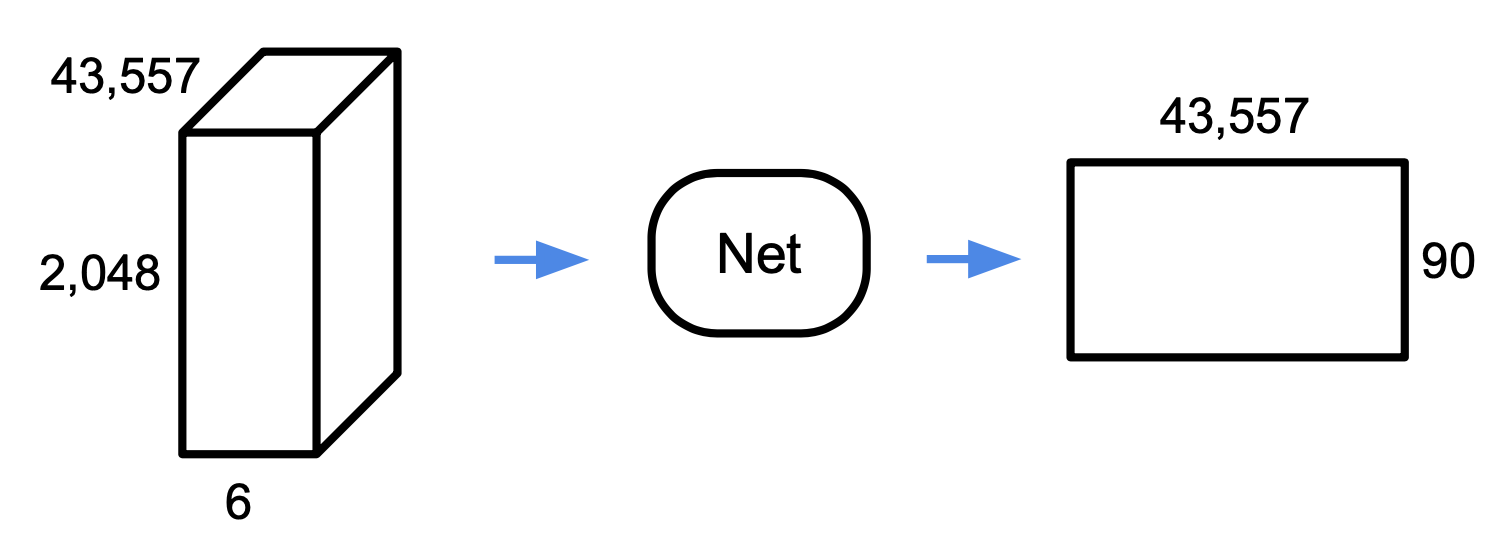
\includegraphics[width=0.8\textwidth]{icu_embedding_method}
\end{center}
\caption{ICD Embedding Method}
\vspace{12px}
To compute an embedding of ICD codes from what the net has learned, 43,557 examples are forward passed through the net producing a 43,557 by 90 matrix.  The 90 rows of this matrix represent 43,557 dimensional embeddings of the ICD codes.
\label{fig:icu_embedding_method}
\end{figure}

\subsection{Semantic Space Inference}

Many ICD codes are highly similar.  For example, consider the possible codes for sepsis conditions.  There are ICD codes for Septic Shock (785.52), Severe Sepsis (995.92), and Septicemia (038), all placed in wildy different places within the taxonomy.  The common ancestor of these codes in the ICD taxonomy, maintained by the World Health Organization, is the root of the entire taxonomy.  If the net predicts code 785.52 but the actual diagnosis is 995.92, the net is penalized.  Maybe the net is generally right about its predictions, but is unreliable at picking the exact ICD code that the doctor happened to pick.  That does seem to be the case.  Specifically, the net appears to be more reliable at detecting the organ that the condition affects.  For example it seems to know if something is wrong with the heart, brain, or liver.  The net's prediction can be visualized as a heat map in a semantic space of ICD codes.  The semantic space self organizes by organ, maybe the most interesting outcome of this work.  See Figure \ref{fig:icu_icd_map}.  It is fascinating that from such simple waveforms, measuring conductivity across the heart (ECG) or optically sensing blood flow in an artery in the finger (PPG), a neural net can develop a sense of which organs are working properly and which are not.

Semantic space embeddings are common in the field of Natural Language Processing, with word2vec being perhaps the most famous \cite{mikolov2013efficient}.

The predictions from before can be used to embed the ICD codes into a lower dimensional space. Remember that just before the final sigmoid, there is an unnormalized representation of the net output.
\begin{gather}
    \mathcal{Z} = \{
        z_{ij},
        \text{ for } i \in \mathcal{I},
        \text{ for } j \in \{ 1, \dots, m \}
    \}
\end{gather}
$\mathcal{Z}$ can be shaped into a matrix $Z$ of size $d \times m |\mathcal{I}|$ where the $d$ rows of this matrix are vector representations of the $d$ ICD Codes.  The dimensionality of these vectors can be reduced from $m |\mathcal{I}|$ to 2 to visualize them.  As with the previous work in dermatology, this can be done using TSNE \cite{van2008visualizing}.

The result of this embedding of ICD codes is shown in Figure \ref{fig:icu_embedding_method}. Conditions are color coded by which part of the body they affect.  Red circles are conditions that affect the heart.  These conditions include cardiogenic shock, coronary atherosclerosis, atrial flutter, systolic heart failure, and myocardial infarction.  Green circles are conditions that affect the brain.  These conditions include cerebral edema, brain cancer, cerebral aneurysm, intracerebral hemorrhage.  It is interesting that skull fracture found its way into this region.  Yellow circles are conditions that affect the liver.  These conditions include cirrhosis, hepatitis, and liver cancer.  It is interesting that alcohol abuse and alcohol dependence syndrome found their way into this region, and are also close to the brain conditions.  Blue circles are conditions that affect the lungs.  These conditions include pulmonary collapse, pneumonia, and acute respiratory failure.  It is remarkable that a highly articulate semantic space can be learned from simple waveforms.  Further similar ICD codes are close together in this semantic space that may be far apart in the ICD taxonomy.  For example, the ICD codes 785.52: Septic Shock, 995.92: Severe Sepsis, and 038: Septicemia.  The nearest common ancestor of these ICD codes in the taxonomy is the root of the entire taxonomy of all medical conditions that exist.  But the net learned that they were similar semantically based on the waveforms it was trained with.

Now that this semantic space and relative risk have been computed for all the test patients, the net's predictions can be visualized on a patient by patient level.  Here the ICD codes are colored according to the risk level that patient has.  Actual diagnoses are circled in white.  See Figures \ref{fig:icu_map_chf}, \ref{fig:icu_map_brain}, \ref{fig:icu_map_liver}.

\begin{figure}
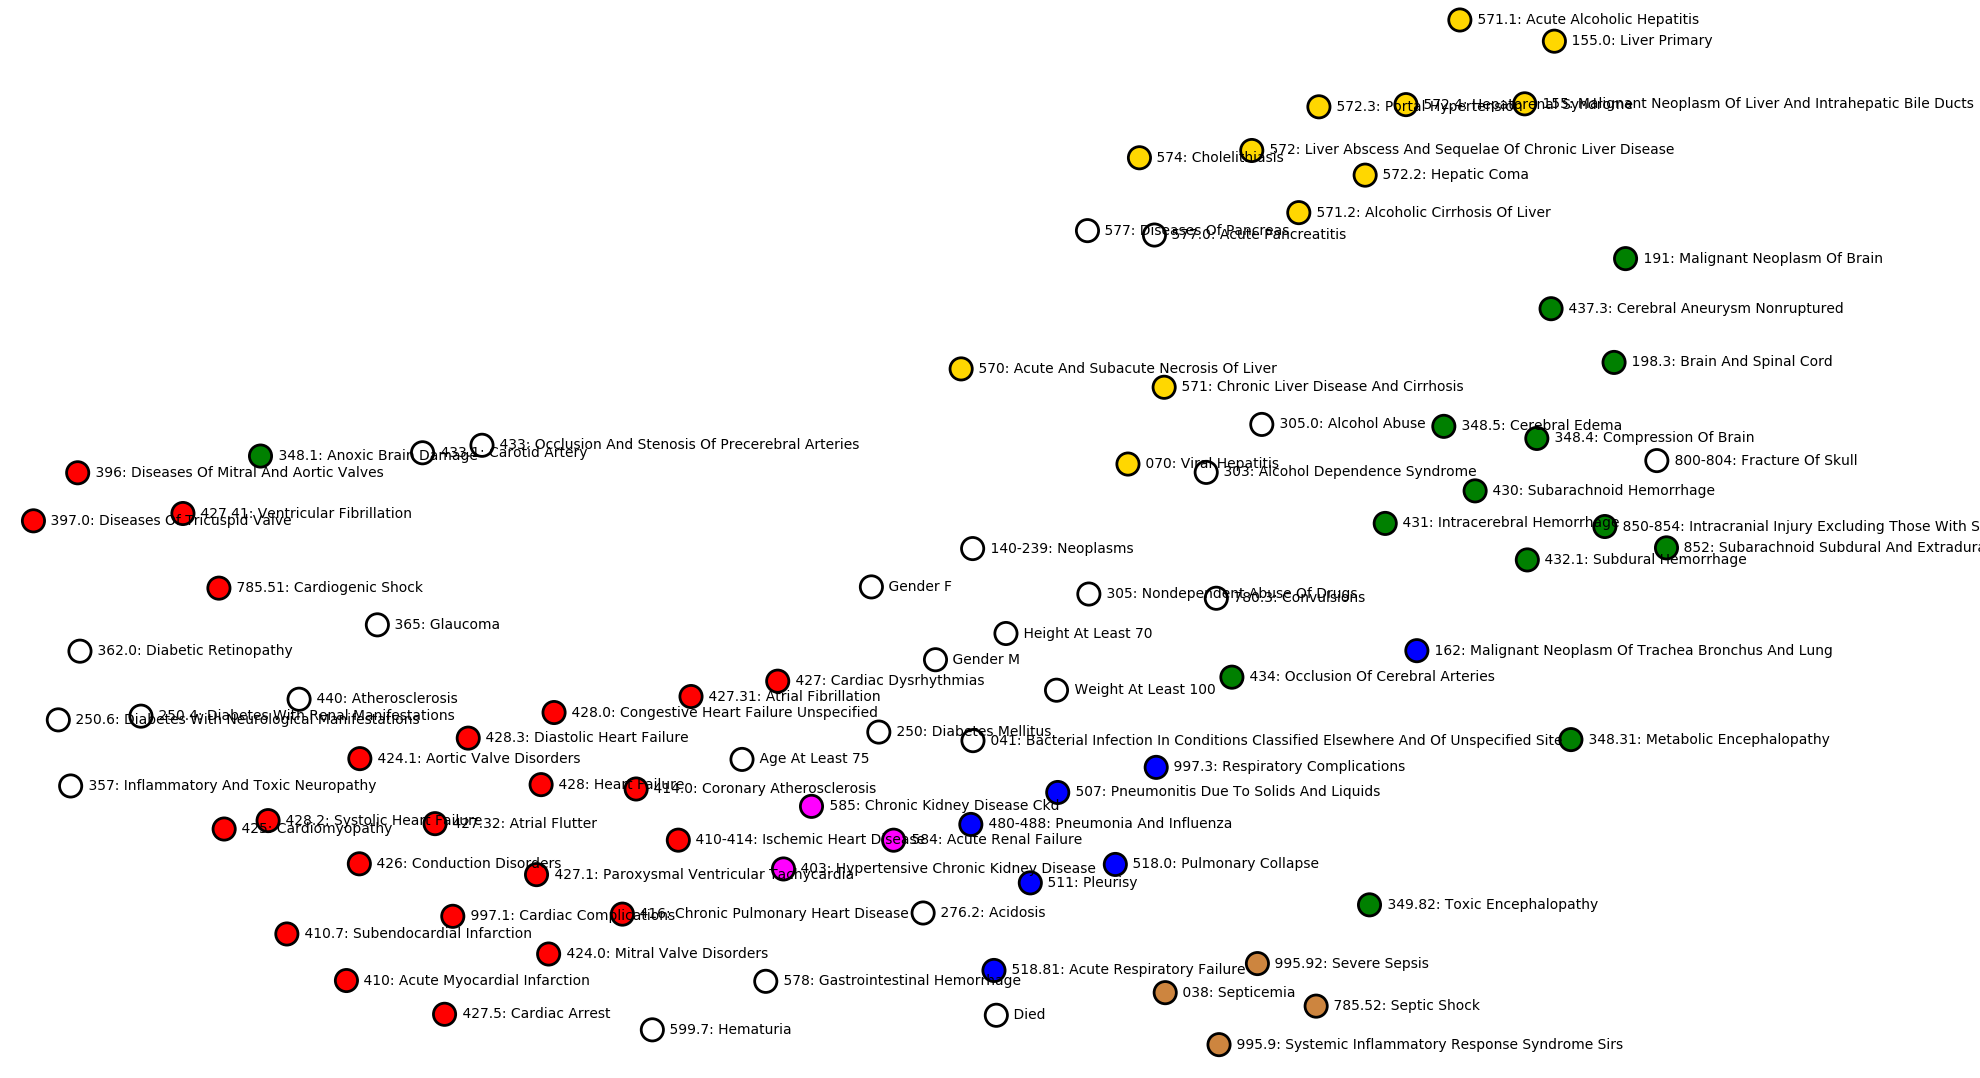
\includegraphics[width=\textwidth]{icu_icd_map}
\caption{ICD Embedding Visualization}
\vspace{12px}
TSNE was applied to high dimensional ICD code embeddings to produce a 2D visualization of the ICD code space learned by the net.  Conditions affecting various organs are close together in this space.  Red circles are conditions that affect the heart.  These conditions include cardiogenic shock, coronary atherosclerosis, atrial flutter, systolic heart failure, and myocardial infarction.  Green circles are conditions that affect the brain.  These conditions include cerebral edema, brain cancer, cerebral aneurysm, intracerebral hemorrhage.  It is interesting that skull fracture found its way into this region.  Yellow circles are conditions that affect the liver.  These conditions include cirrhosis, hepatitis, and liver cancer.  It is interesting that alcohol abuse and alcohol dependence syndrome found their way into this region, and are also close to the brain conditions.  Blue circles are conditions that affect the lungs.  These conditions include pulmonary collapse, pneumonia, and acute respiratory failure.  This embedding also puts similar ICD codes together that may be far apart in the ICD taxonomy.  For example consider ICD code 785.52: Septic Shock, ICD code 995.92: Severe Sepsis, and ICD code 038: Septicemia.  The nearest common ancestor of these ICD codes in the taxonomy is the root of the entire taxonomy of all medical conditions that exist.  But the net learned that they were similar semantically based on the waveforms it was trained with.
\label{fig:icu_icd_map}
\end{figure}
    
\begin{figure}
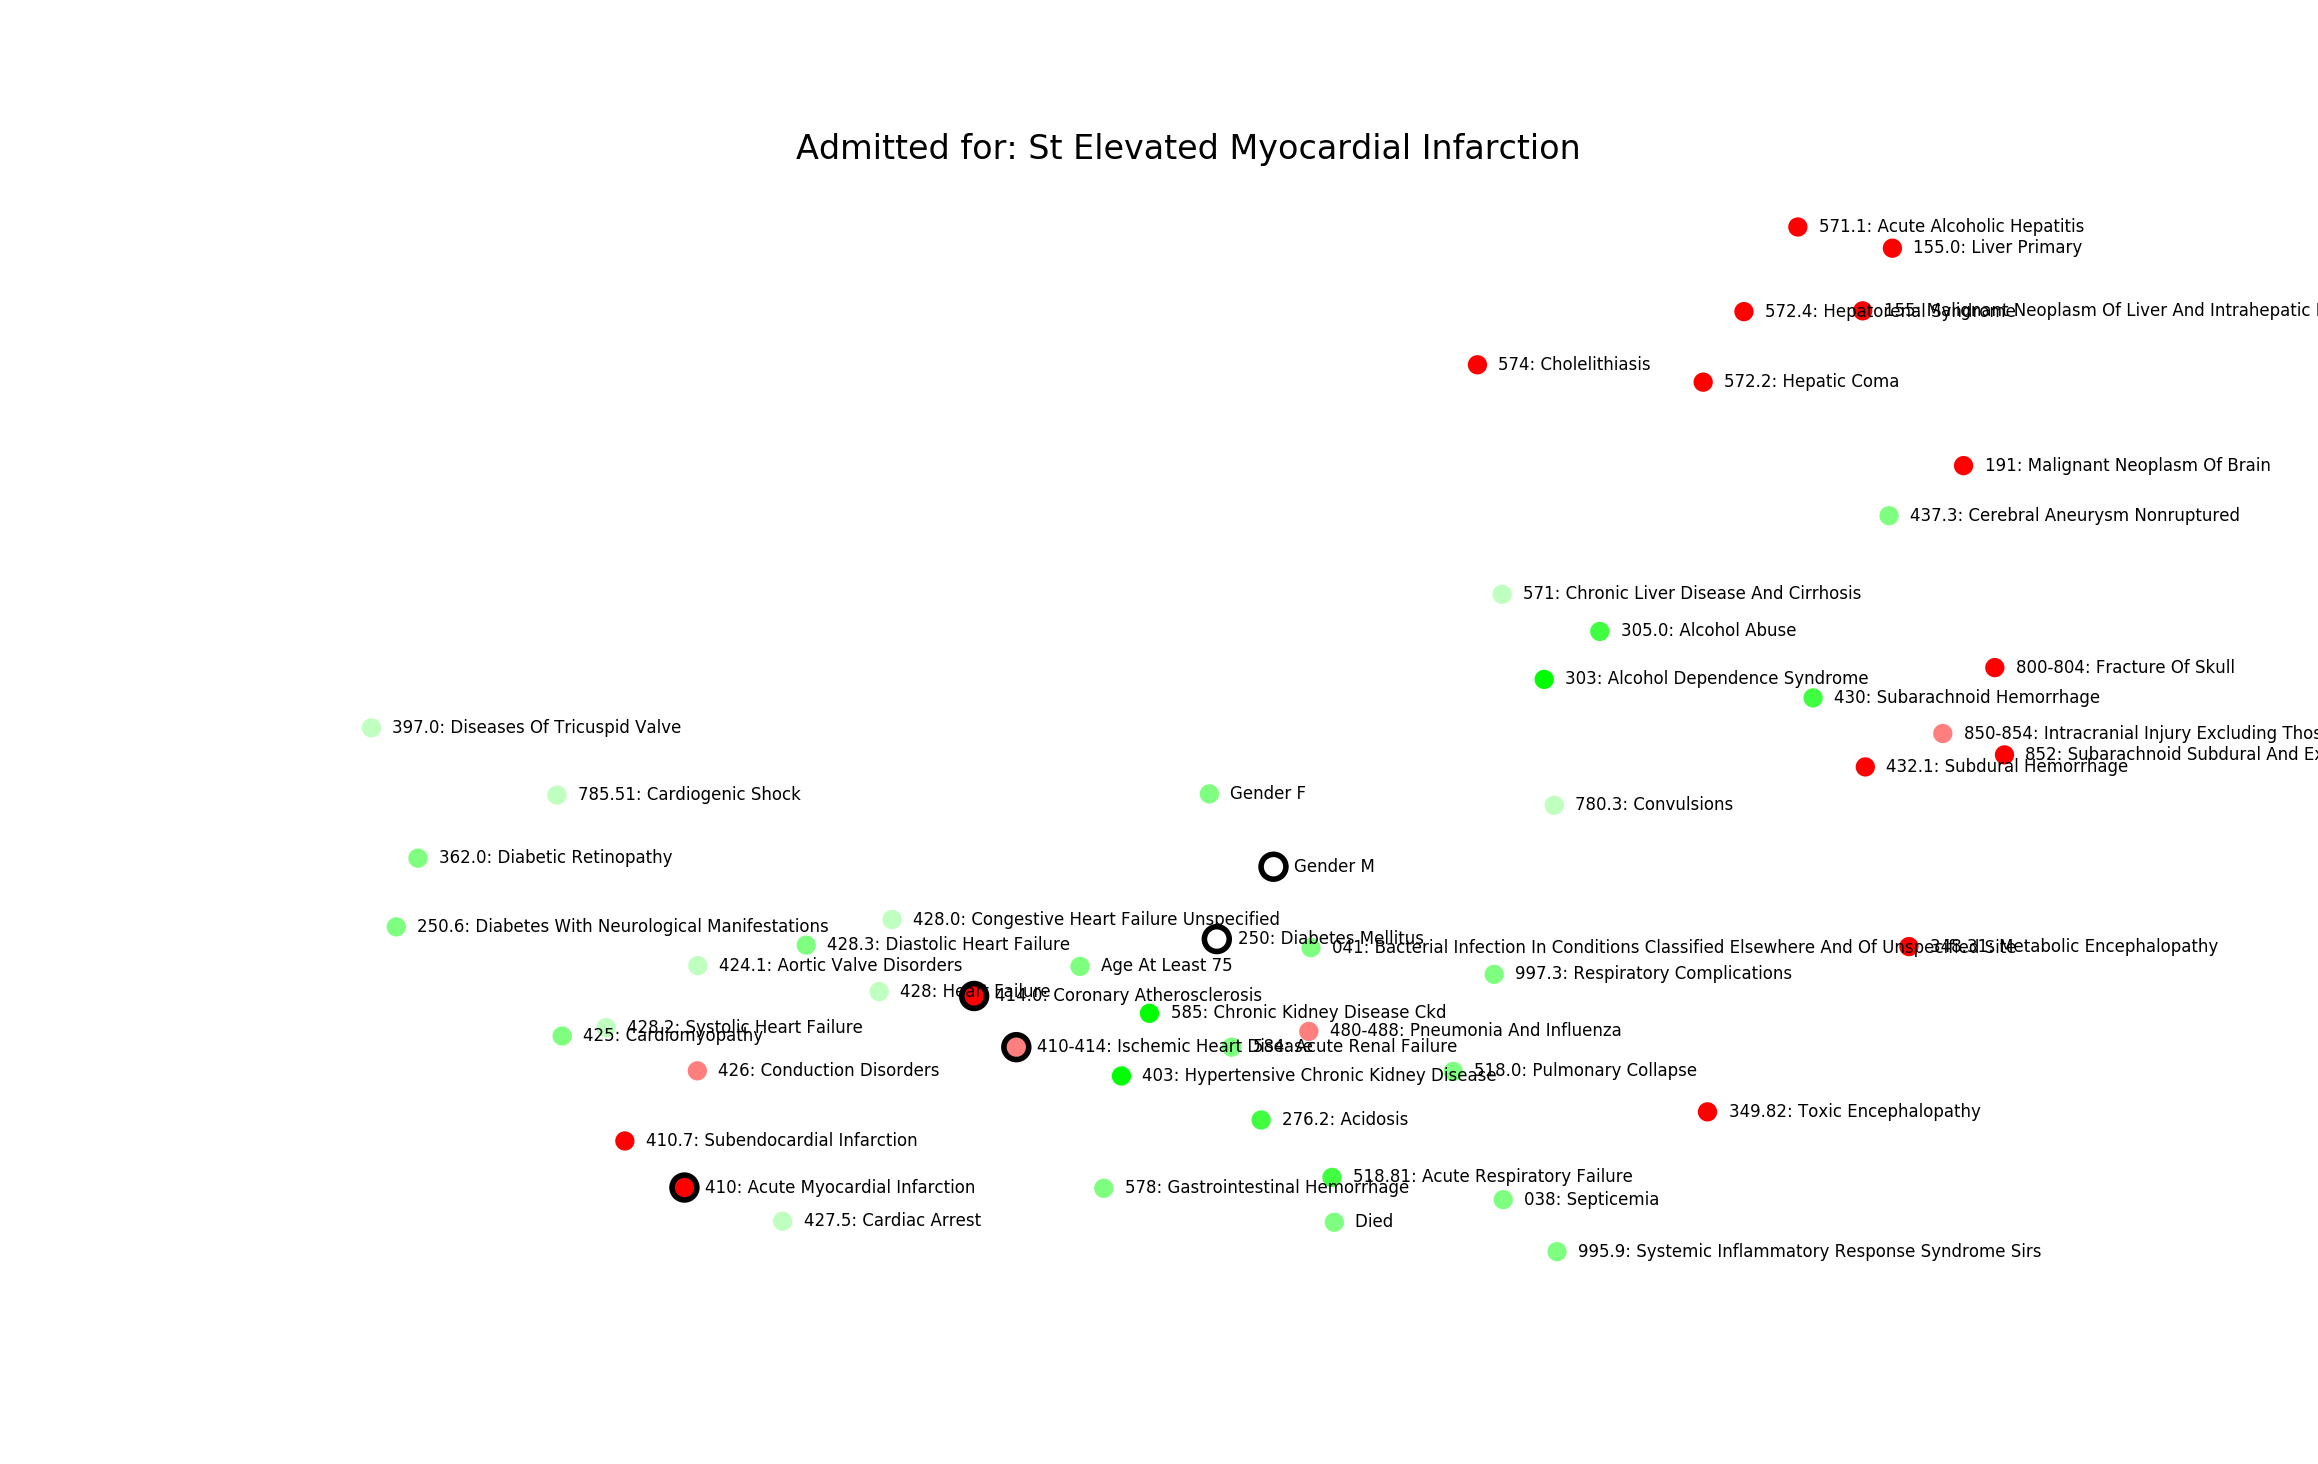
\includegraphics[width=\textwidth]{icu_map_mi}
\caption{Semantic Inference Myocardial Infarction}
\vspace{12px}
This patient was admitted for ``ST Elevated Myocardial Infarction".  The neural net correctly predicted that they had low risk of kidney conditions, death, and many heart conditions (colored green).  It predicted high risk of liver conditions and various heart conditions including myocardial infarction and coronary atherosclerosis (colored red).  The patient was eventually in fact diagnosed with myocardial infarction and coronary atherosclerosis among other things (circled in black).
\label{fig:icu_map_mi}
\end{figure}

\begin{figure}
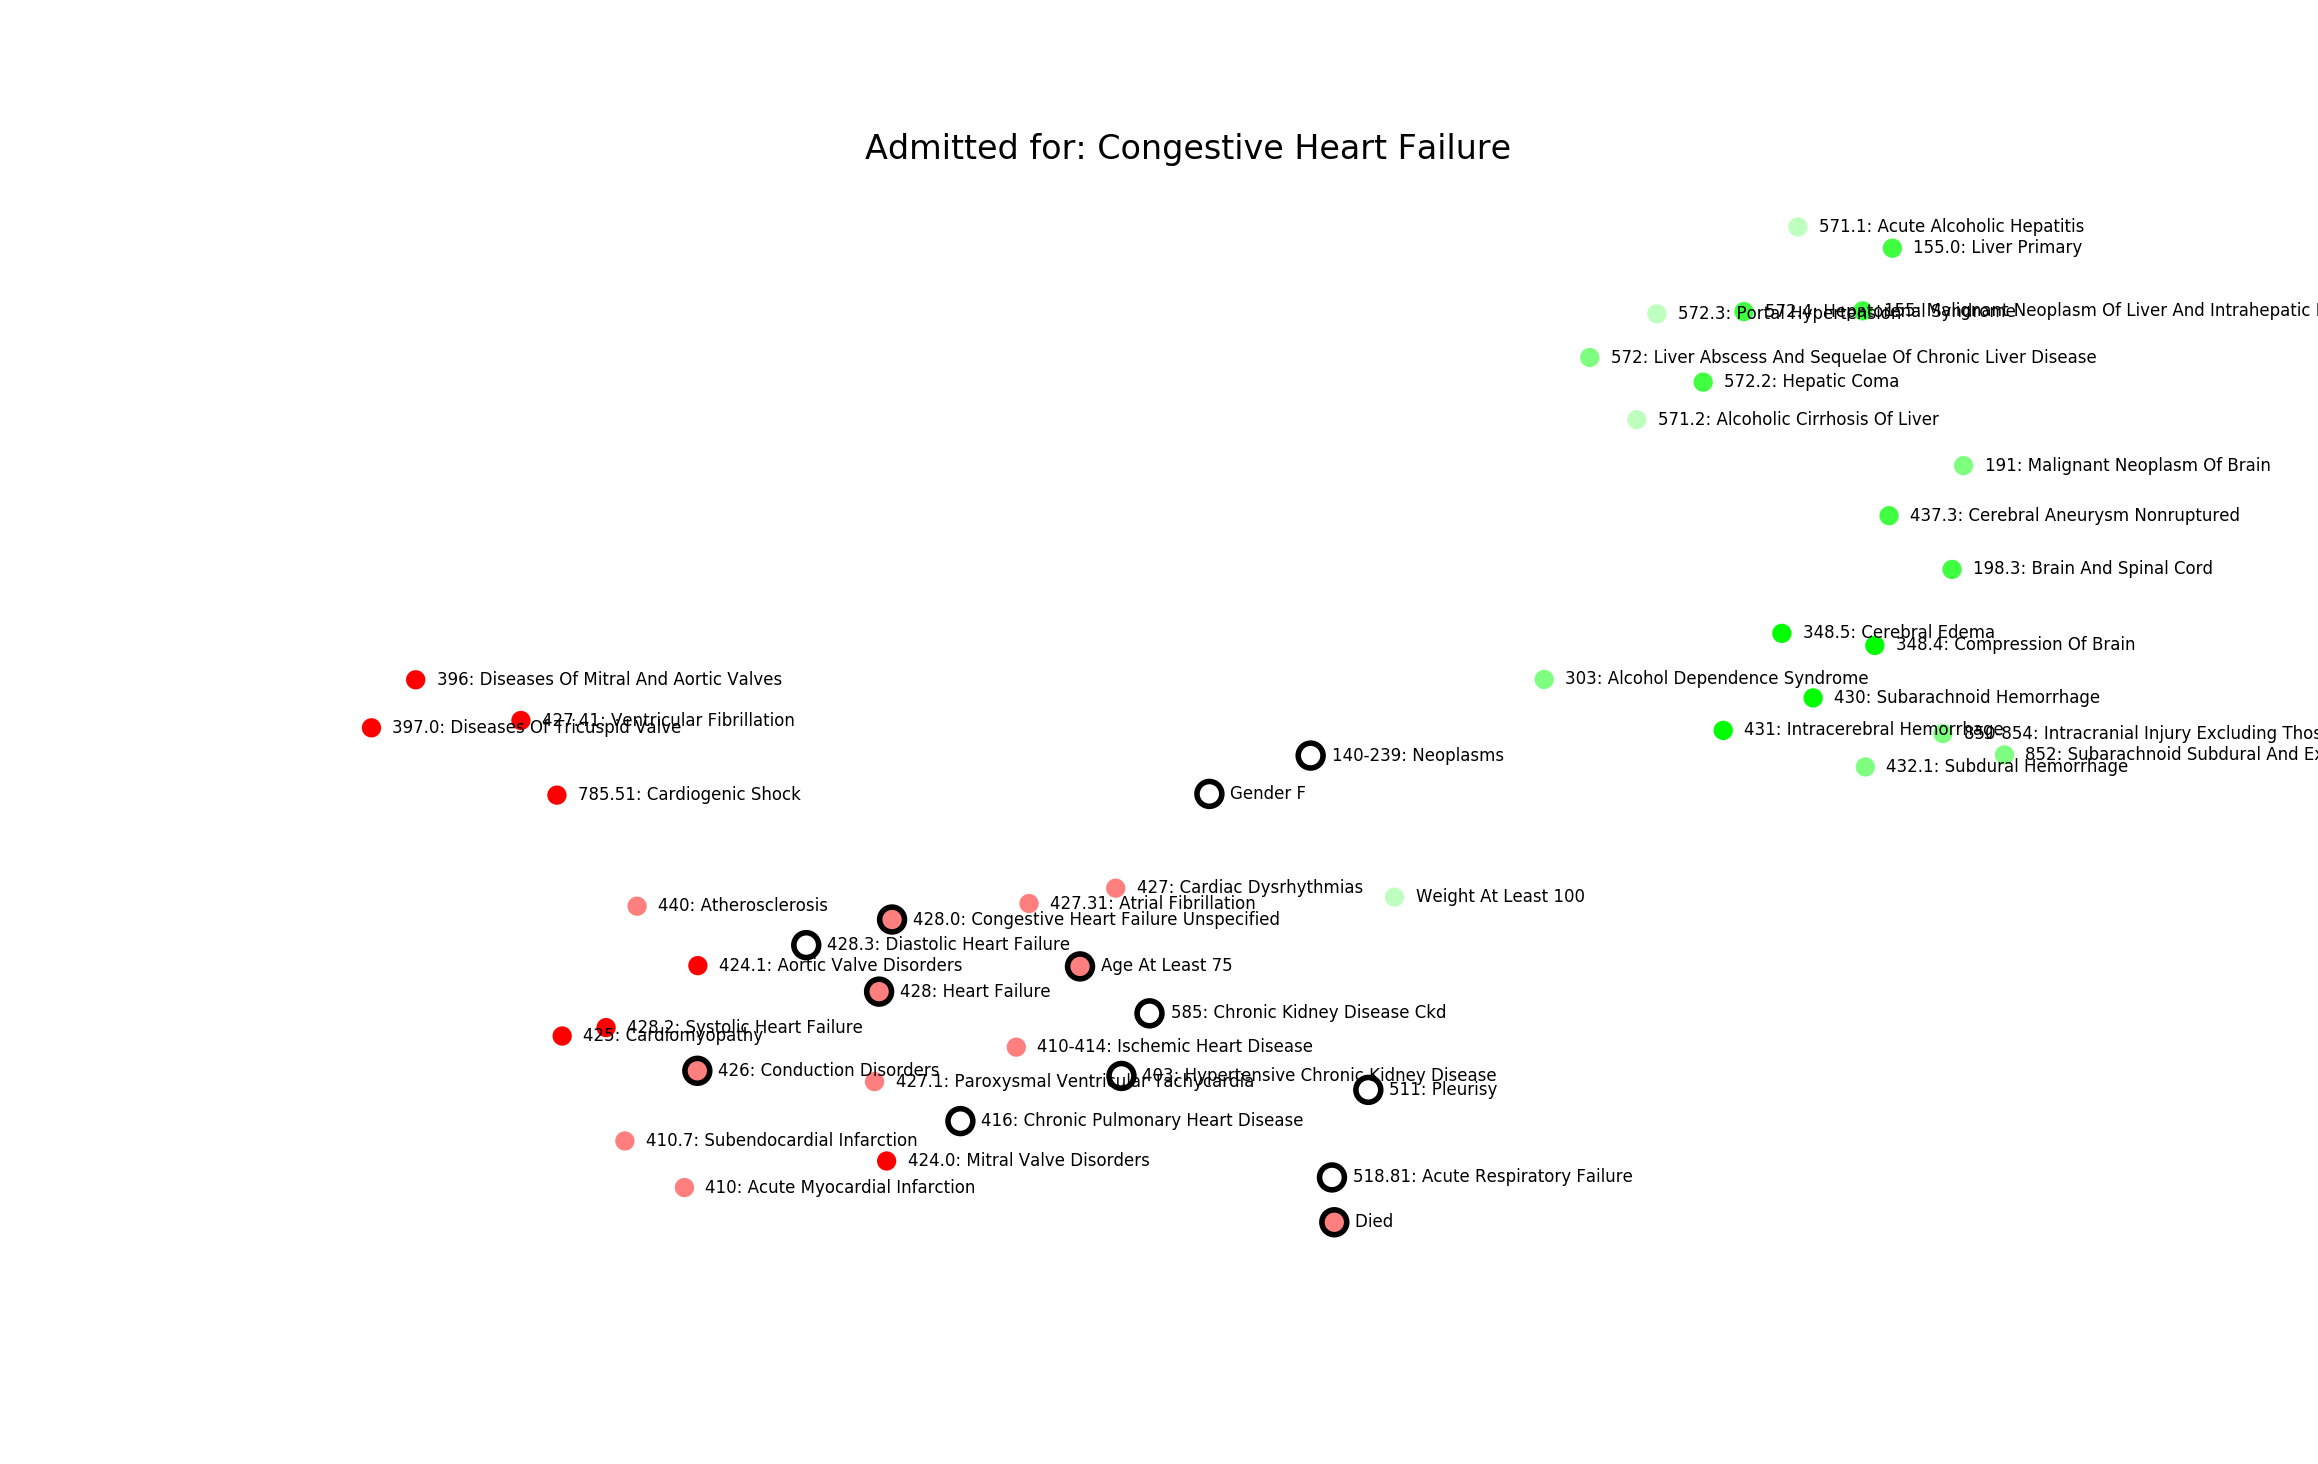
\includegraphics[width=\textwidth]{icu_map_chf}
\caption{Semantic Inference Congestive Heart Failure}
\vspace{12px}
This patient was admitted for ``Congestive Heart Failure".  The neural net predicted that they had low risk of liver and brain conditions (colored green).  It predicted high risk of heart conditions (colored red).  The patient was eventually diagnosed of conditions affecting the heart, and died (circled in black).
\label{fig:icu_map_chf}
\end{figure}

\begin{figure}
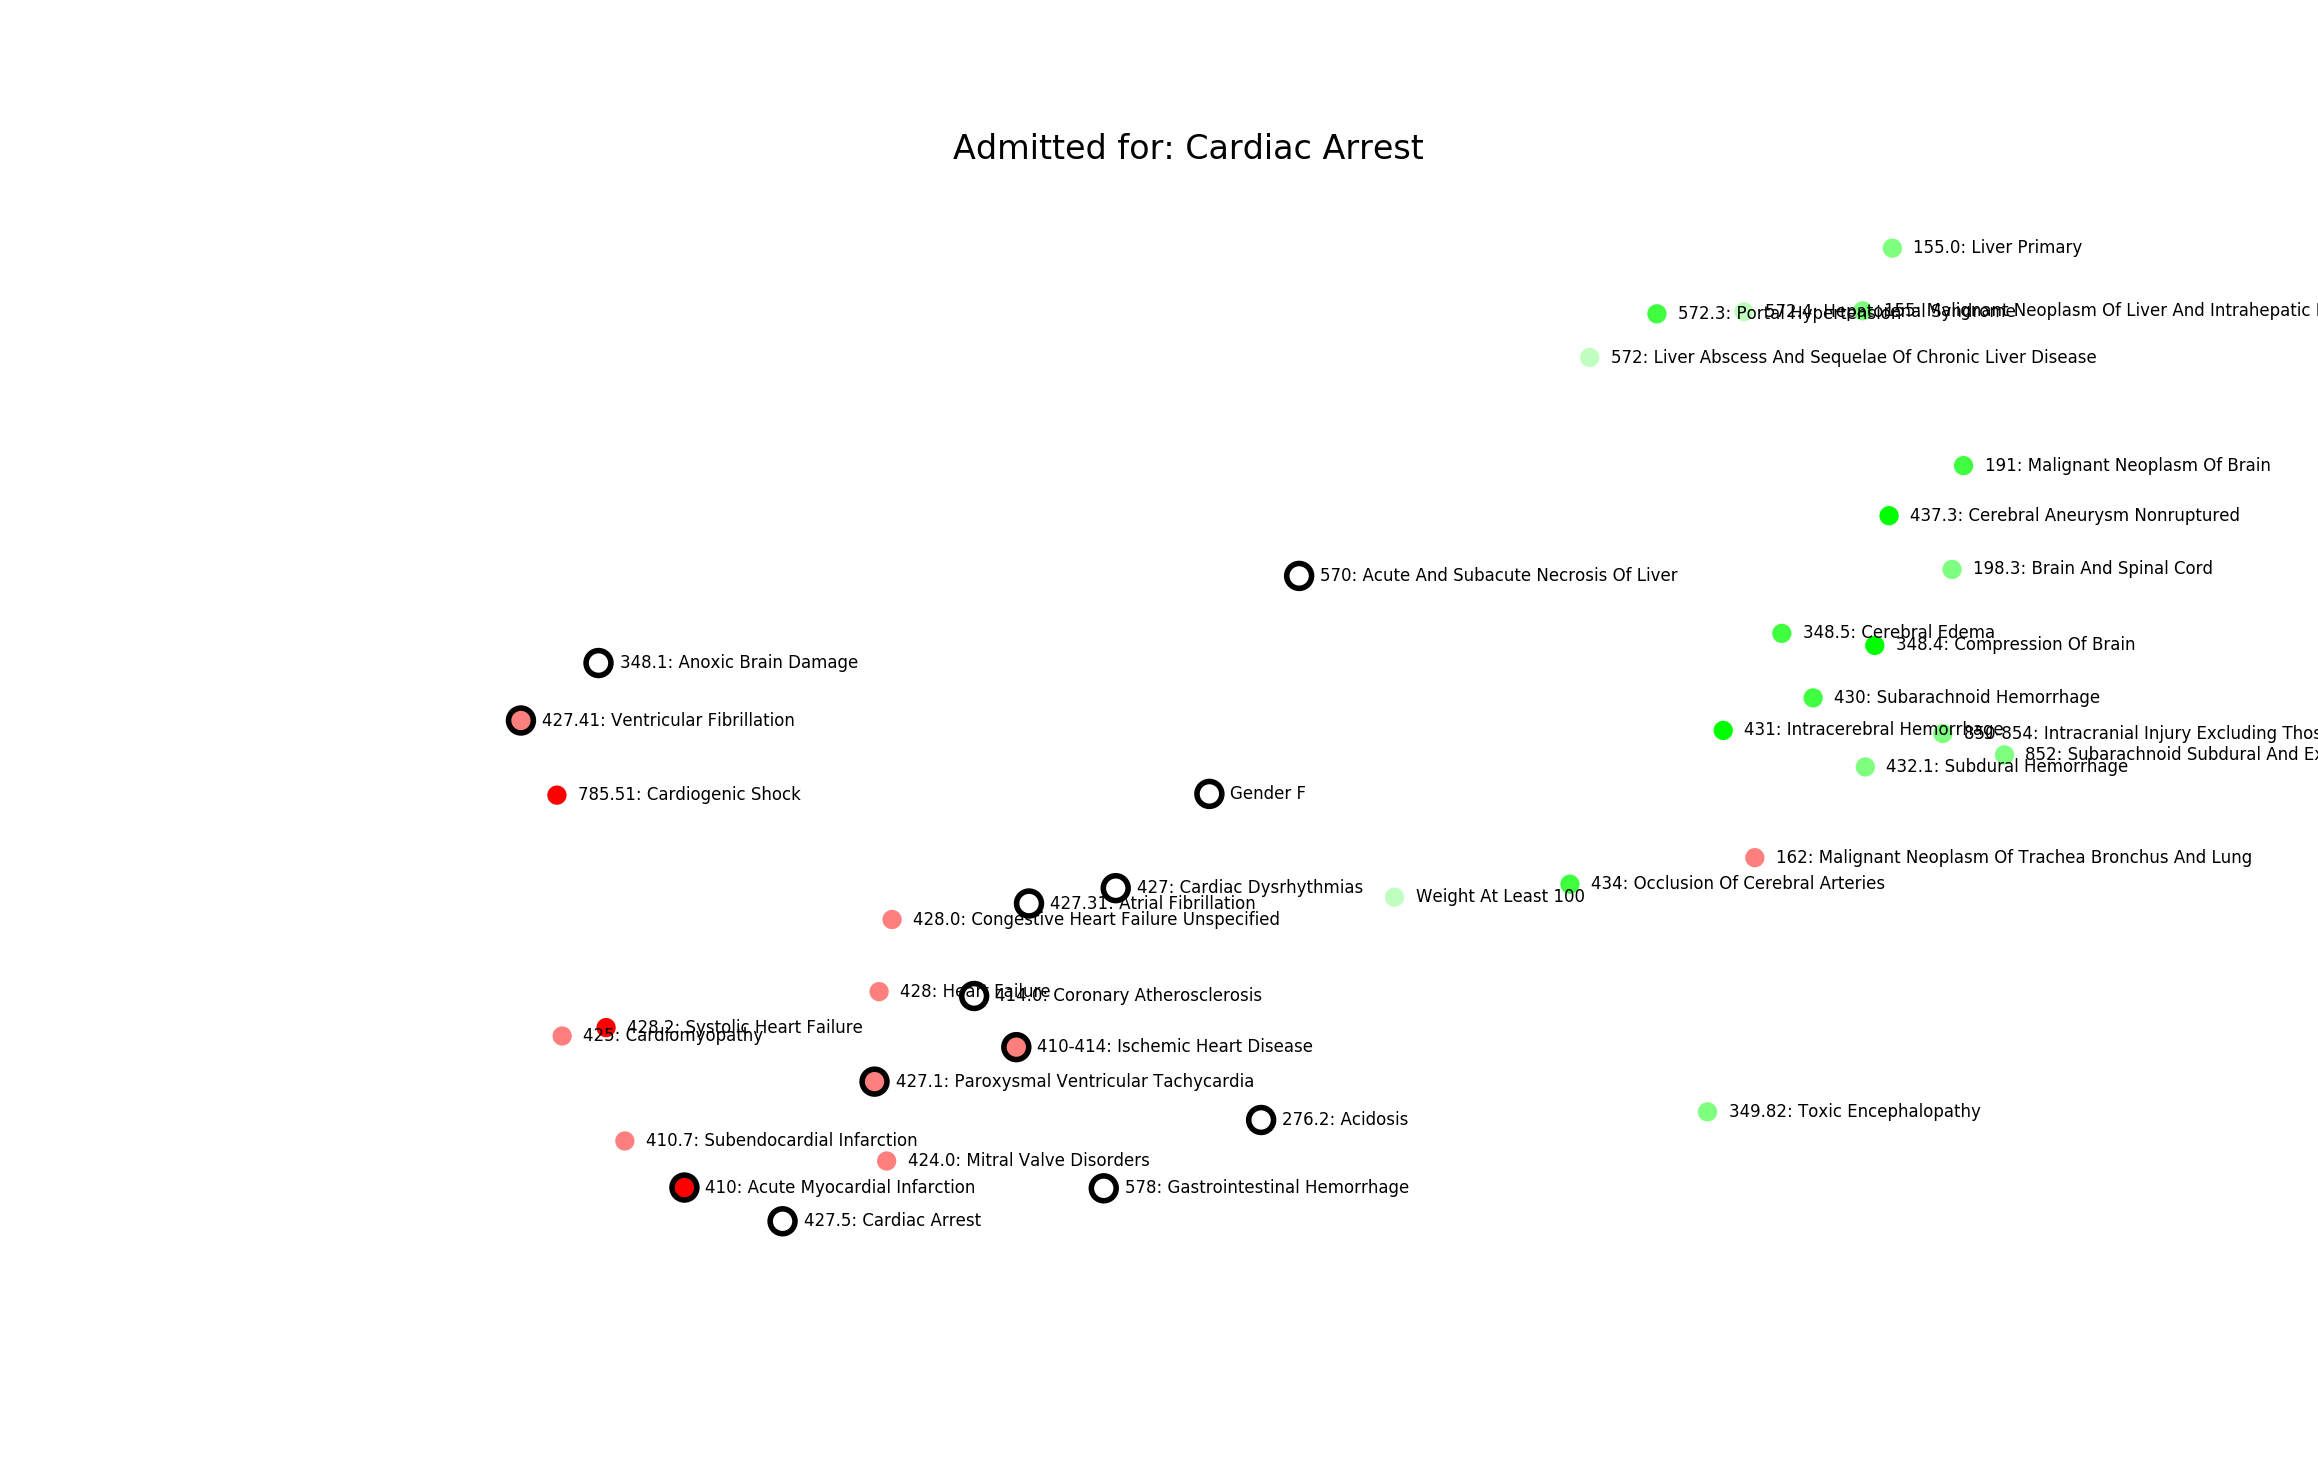
\includegraphics[width=\textwidth]{icu_map_cardarr}
\caption{Semantic Inference Cardiac Arrest}
\vspace{12px}
This patient was admitted for ``Cardiac Arrest".  The neural net predicted that they had low risk of liver and brain conditions (colored green).  It predicted high risk of heart conditions (colored red).  The patient was eventually diagnosed of conditions affecting the heart among other things (circled in black).
\label{fig:icu_map_cardarr}
\end{figure}

\begin{figure}
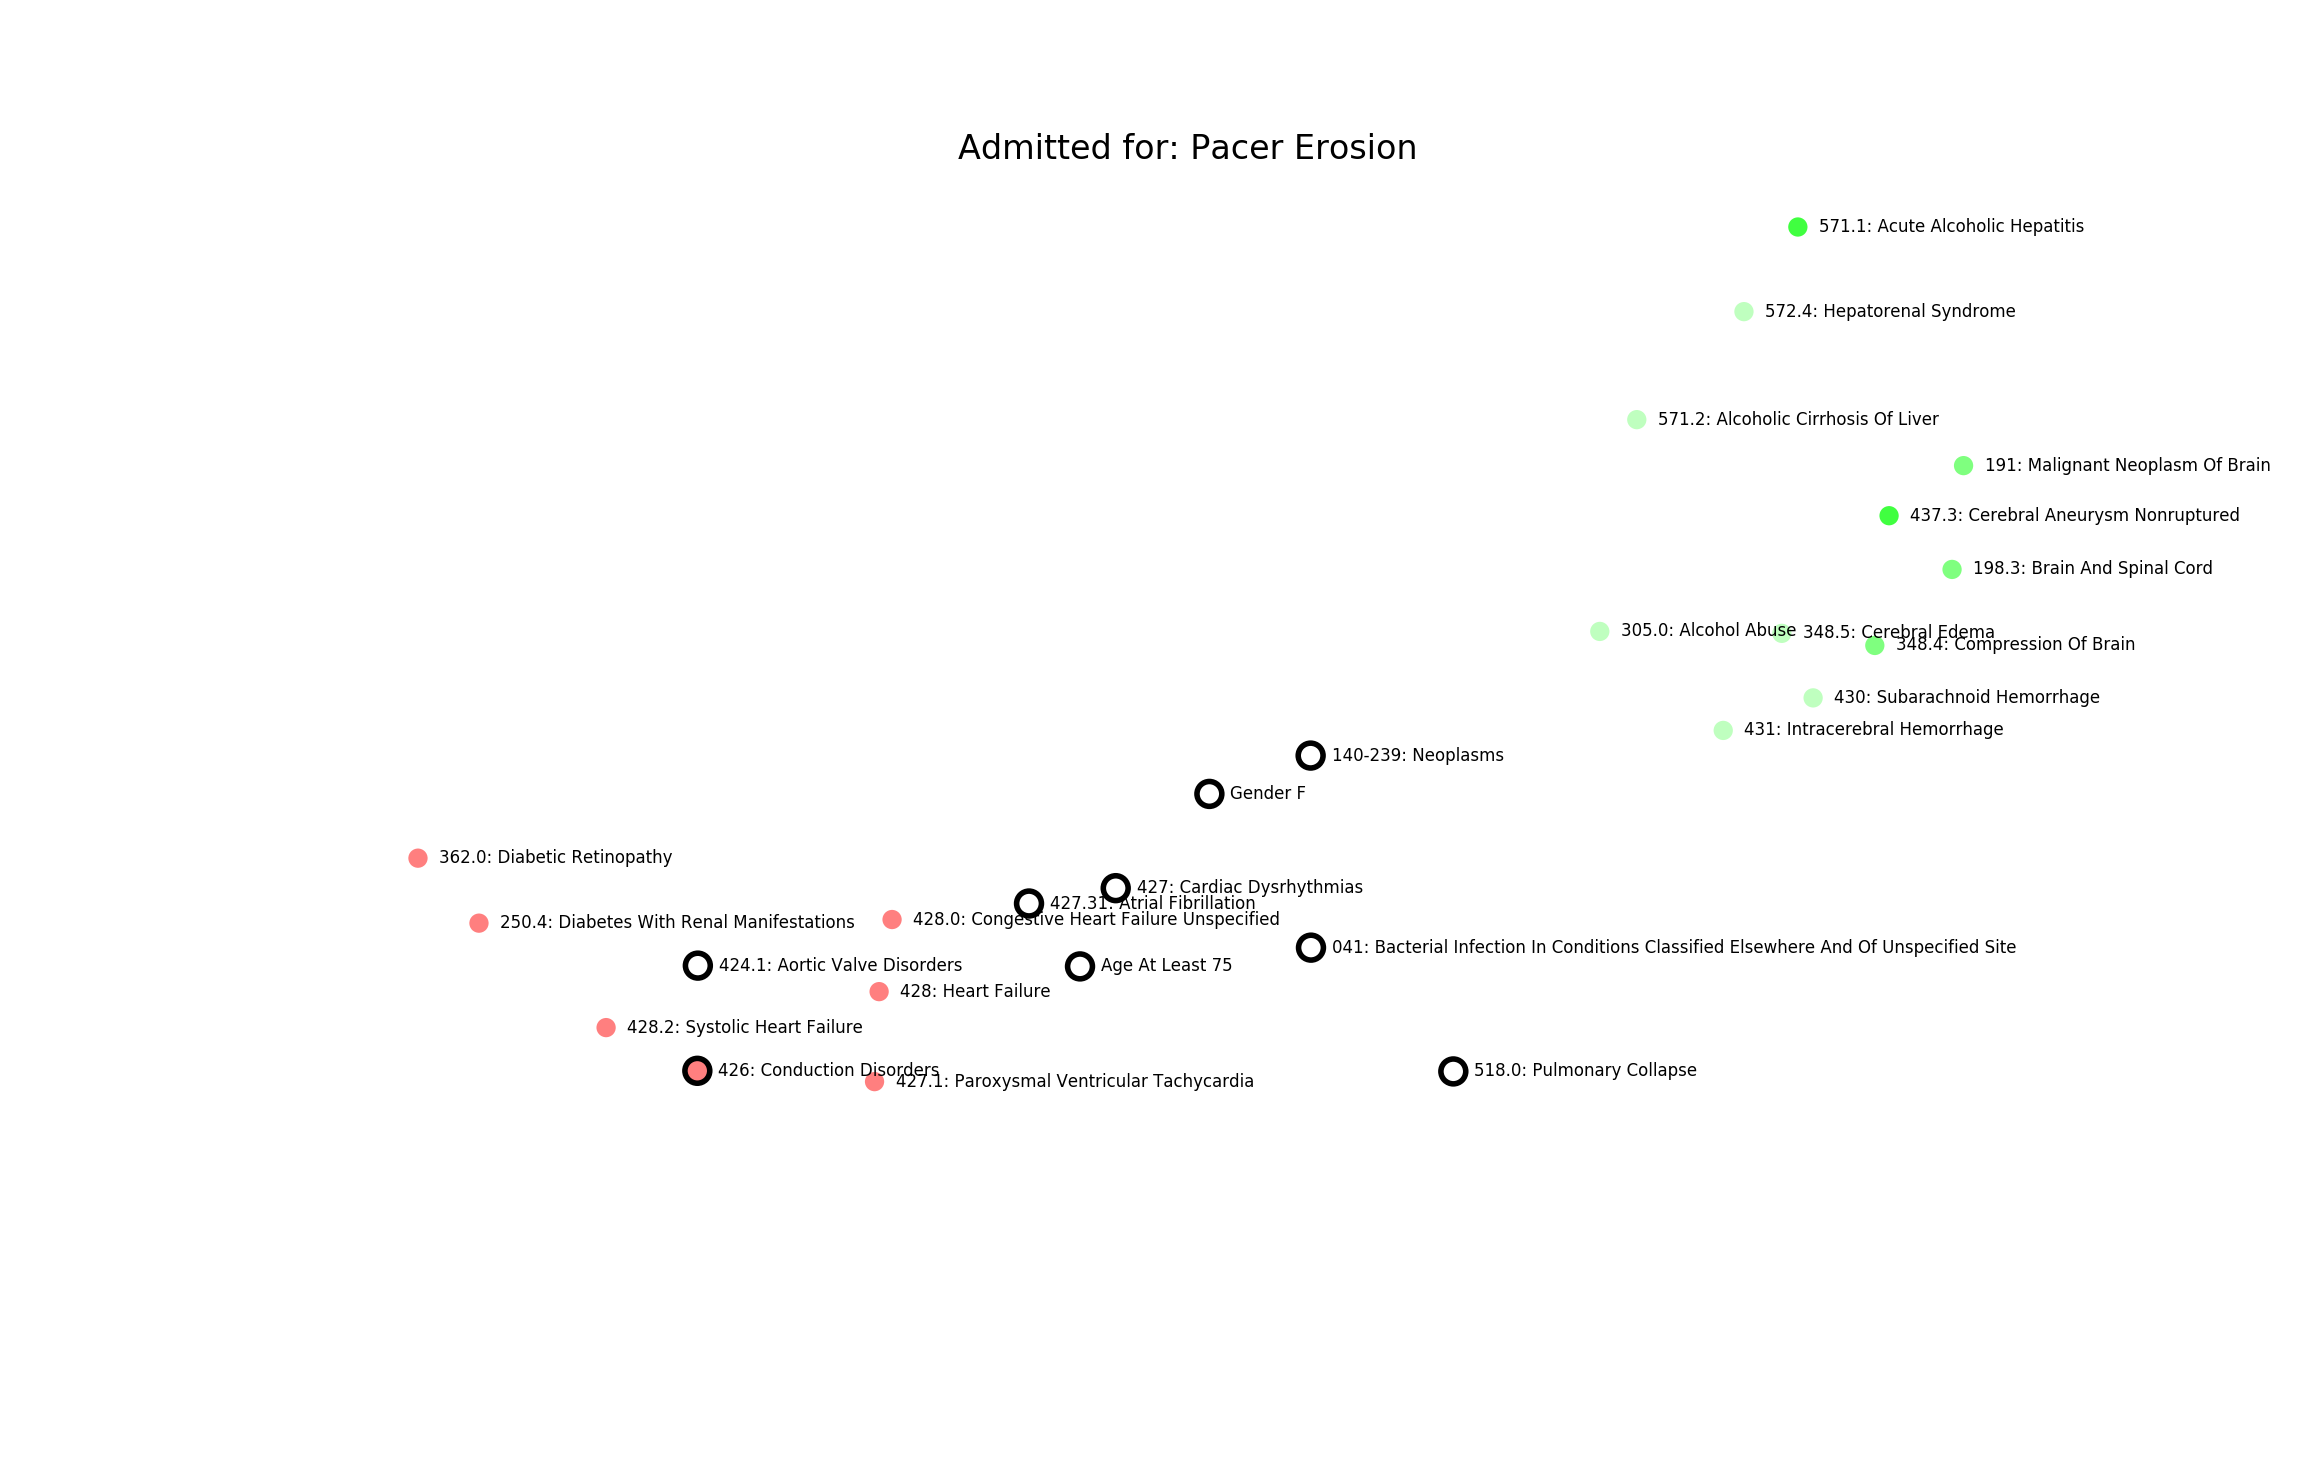
\includegraphics[width=\textwidth]{icu_map_pacer}
\caption{Semantic Inference Pacer Erosion}
\vspace{12px}
This patient was admitted for ``Pacer Erosion".  The neural net predicted that they had low risk of liver and brain conditions (colored green).  It predicted high risk of heart conditions (colored red).  The patient was eventually diagnosed of conditions affecting the heart (circled in black).
\label{fig:icu_map_pacer}
\end{figure}

\begin{figure}
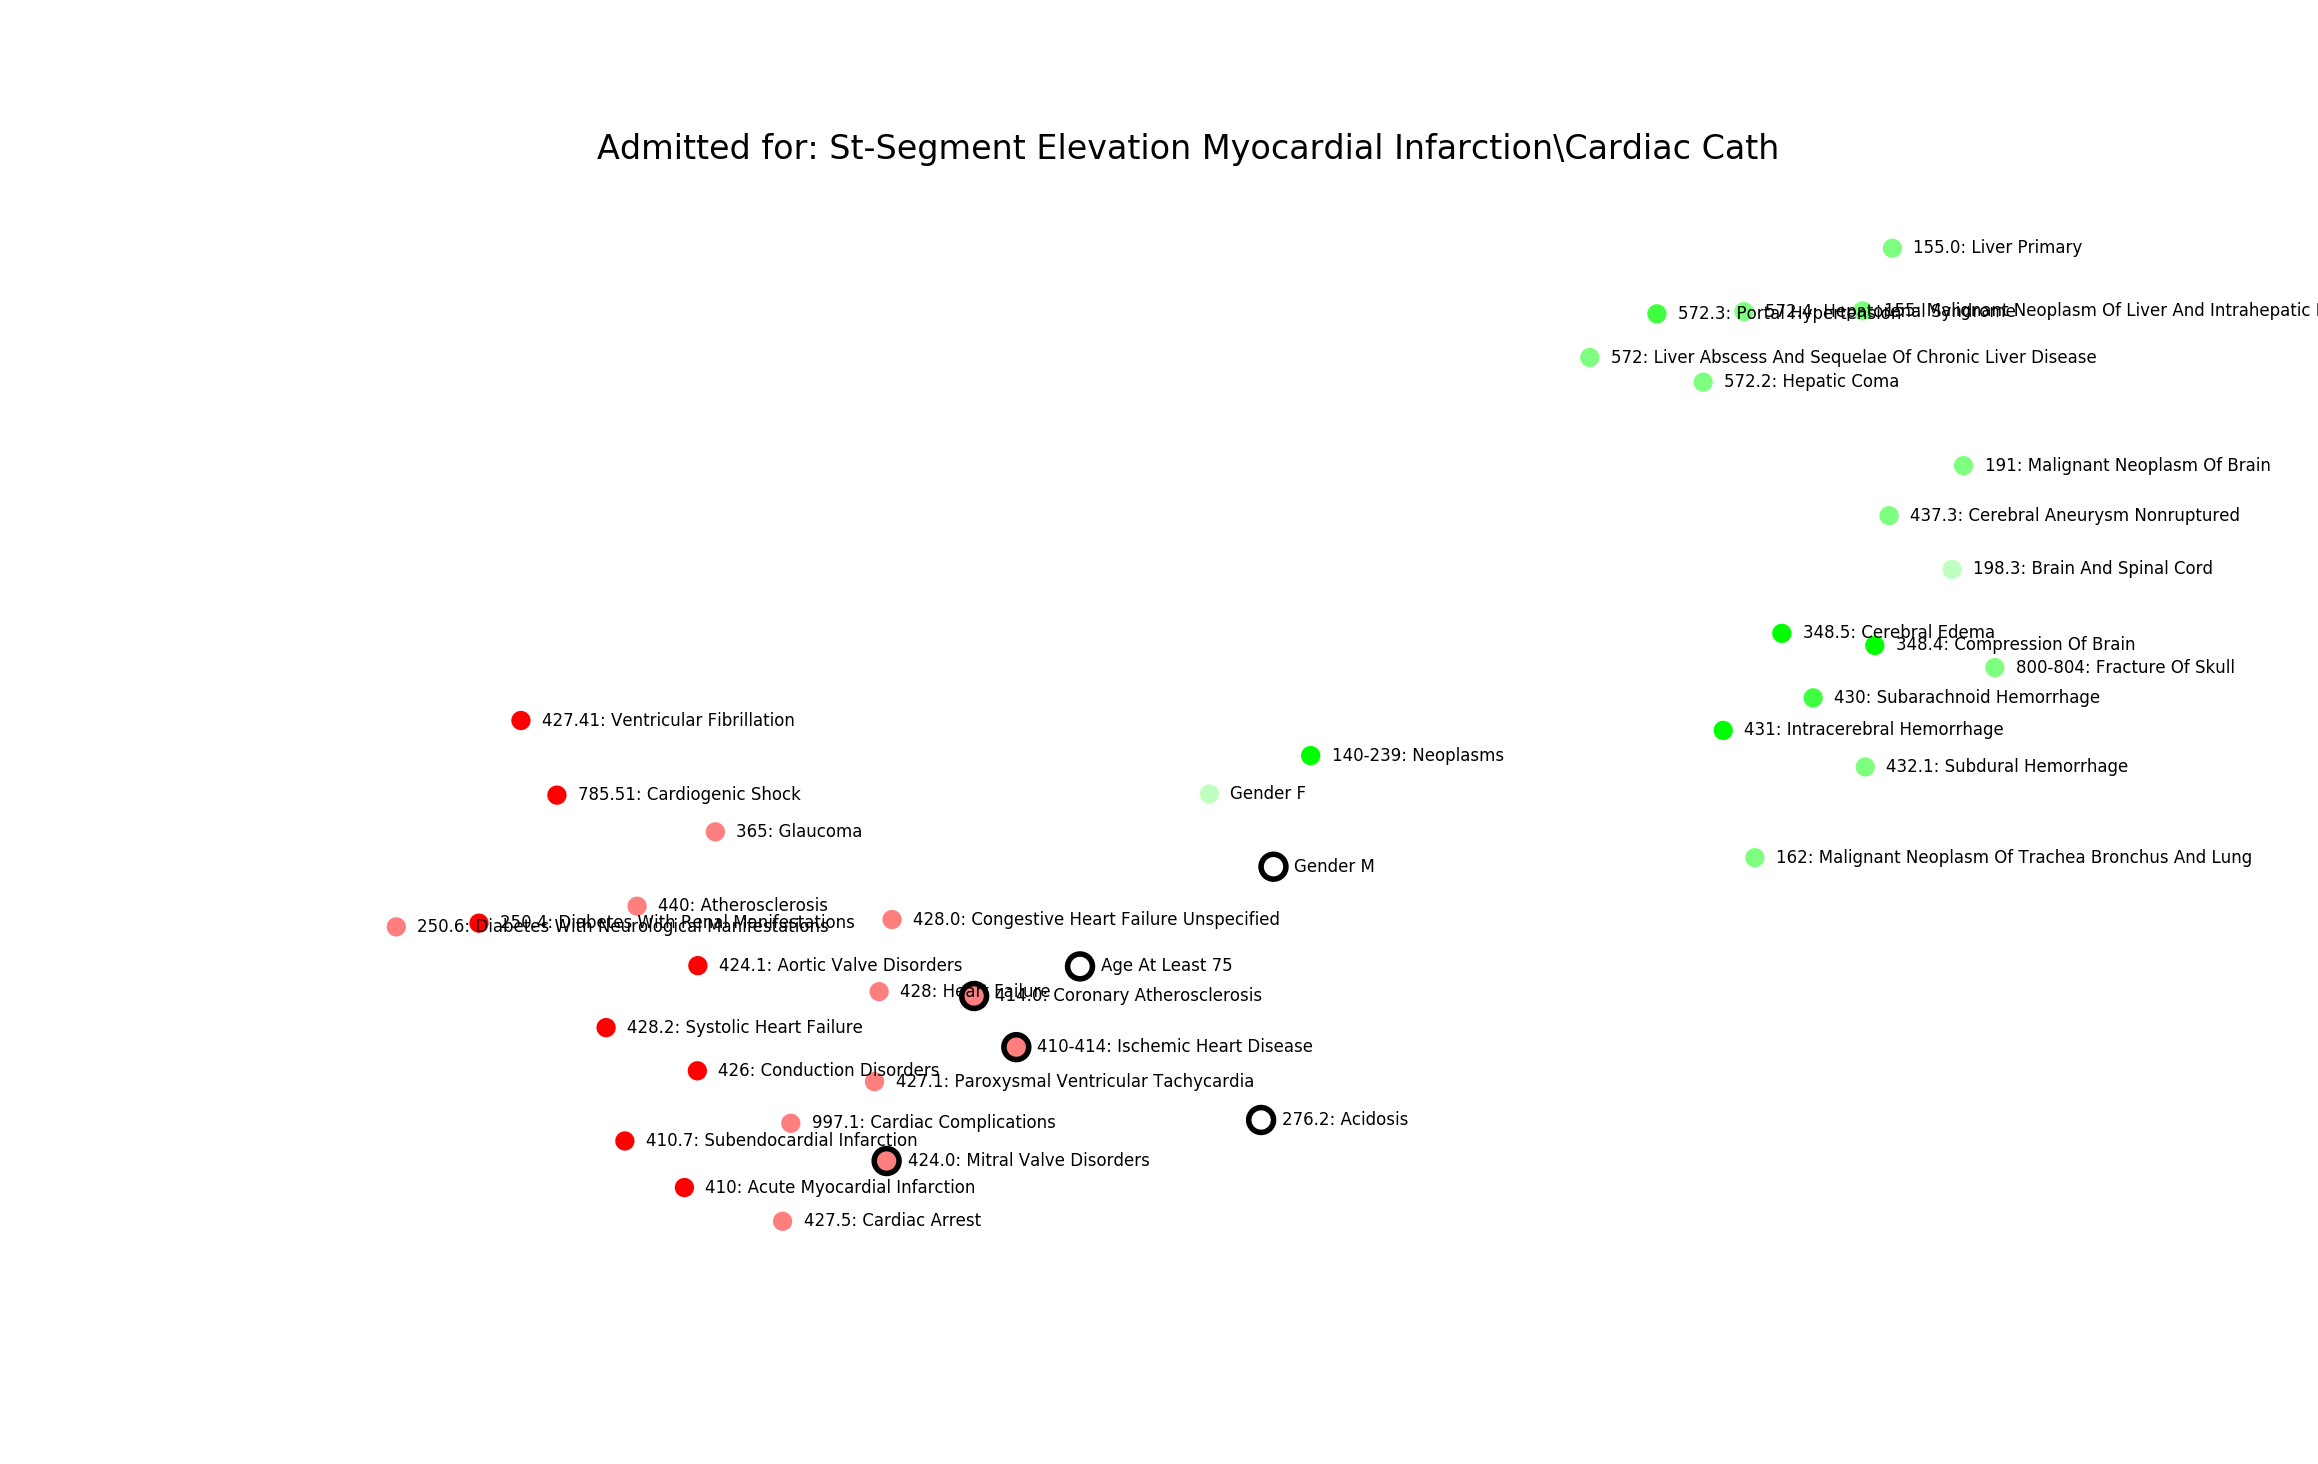
\includegraphics[width=\textwidth]{icu_map_stseg}
\caption{Semantic Inference ST Elevation}
\vspace{12px}
This patient was admitted for ``St-Segment Elevation Myocardial Infarction/Cardiac Cath".  The neural net predicted that they had low risk of liver and brain conditions (colored green).  It predicted high risk of heart conditions (colored red).  The patient was eventually diagnosed of conditions affecting the heart (circled in black).
\label{fig:icu_map_stseg}
\end{figure}

\begin{figure}
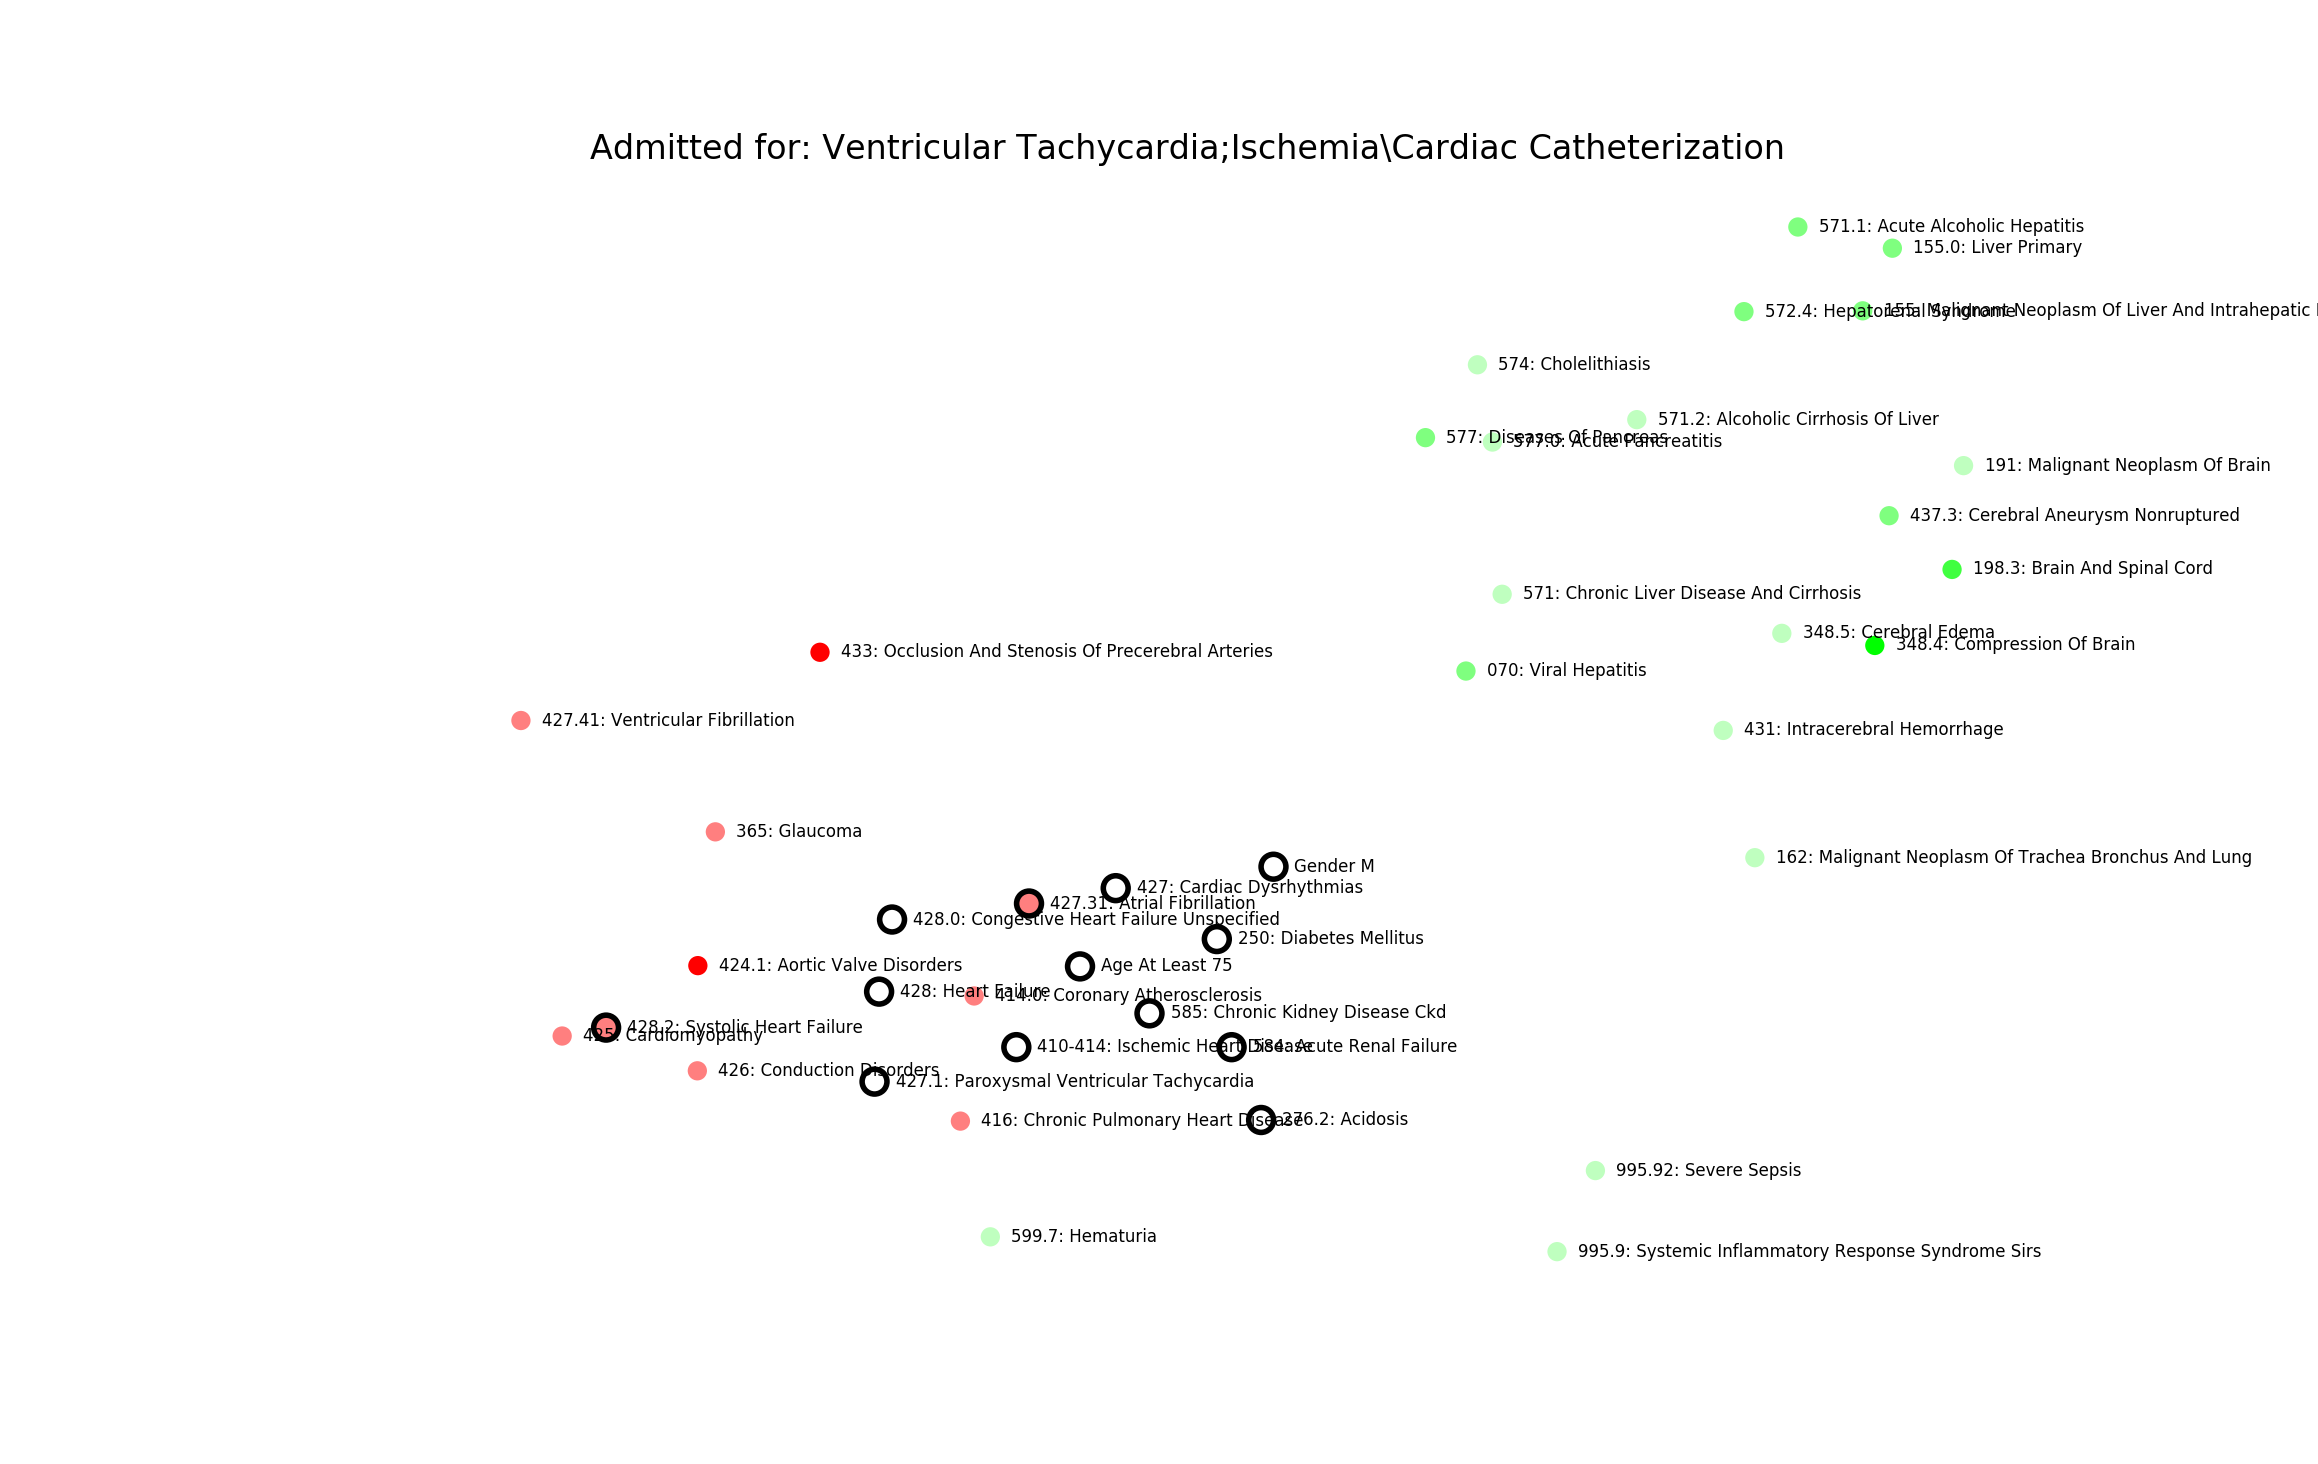
\includegraphics[width=\textwidth]{icu_map_ventach}
\caption{Semantic Inference Ventricular Tachycardia}
\vspace{12px}
This patient was admitted for ventricular tachycardia.  The neural net predicted that they had low risk of liver and brain conditions (colored green).  It predicted high risk of heart conditions (colored red).  The patient was eventually diagnosed of conditions affecting the heart (circled in black).
\label{fig:icu_map_ventach}
\end{figure}

\begin{figure}
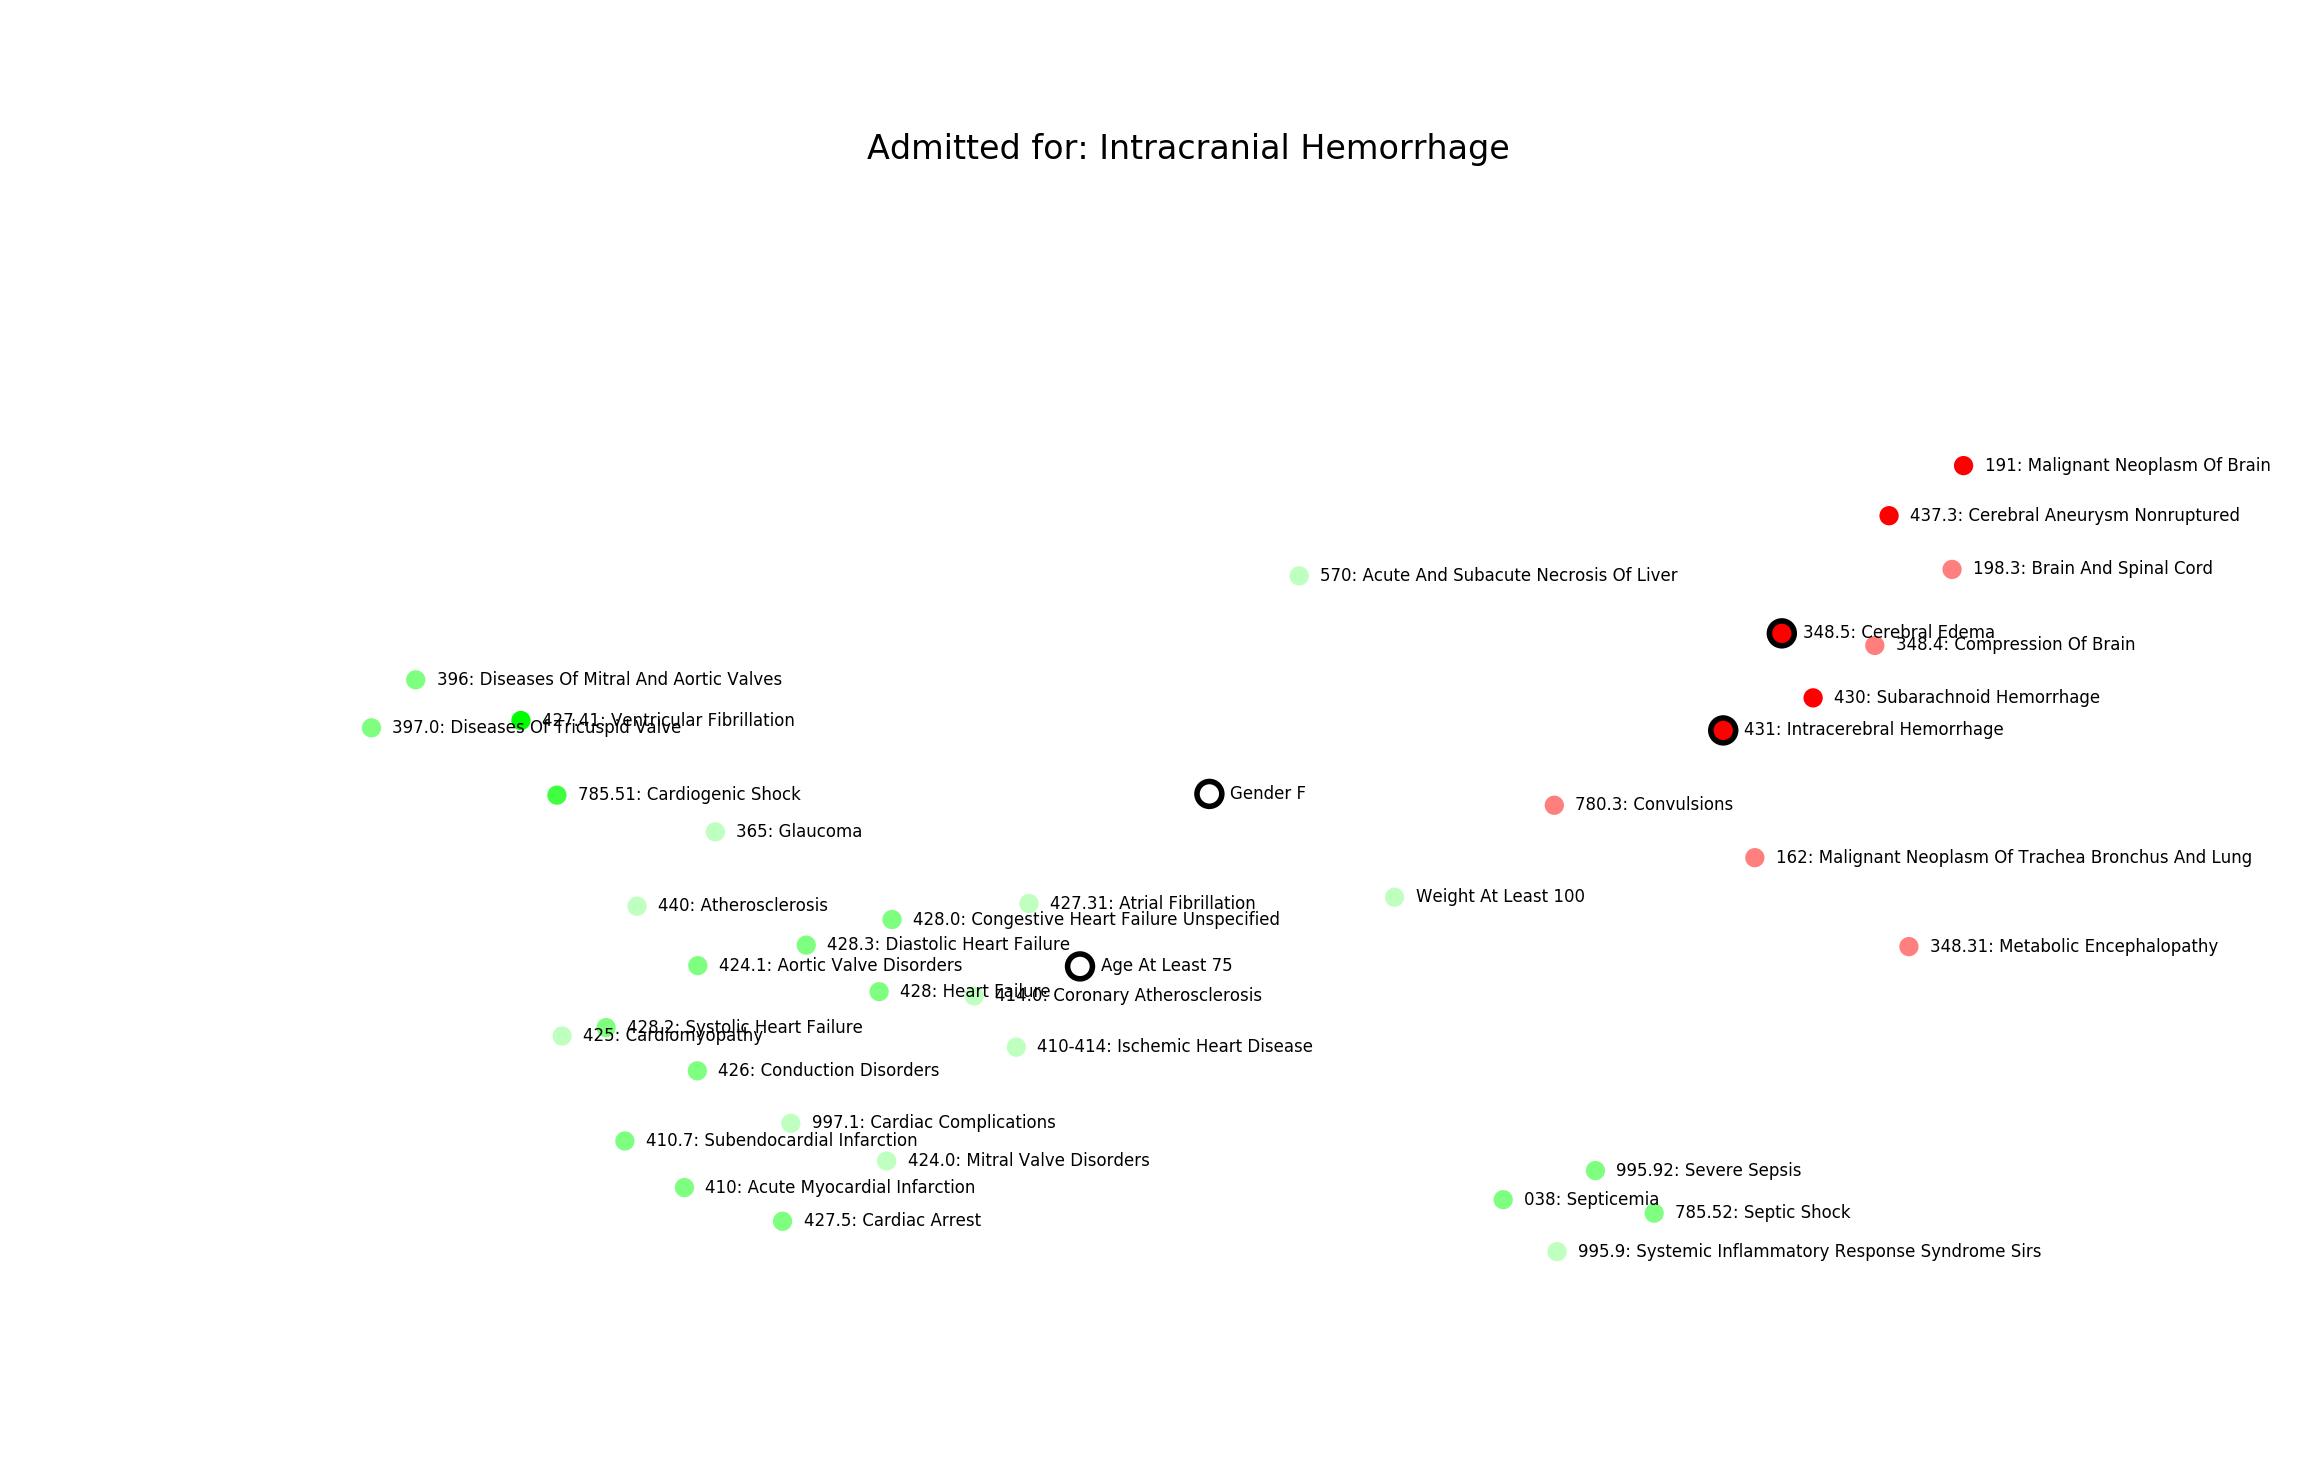
\includegraphics[width=\textwidth]{icu_map_brain}
\caption{Semantic Inference Intracranial Hemorrhage}
\vspace{12px}
This patient was admitted for ``Intracranial Hemorrhage".  The neural net predicted that they had low risk of heart conditions and septic conditions (colored green).  It predicted high risk of brain conditions (colored red).  The patient was eventually diagnosed with cerebral edema and intracerebral hemorrhage (circled in black).
\label{fig:icu_map_brain}
\end{figure}

\begin{figure}
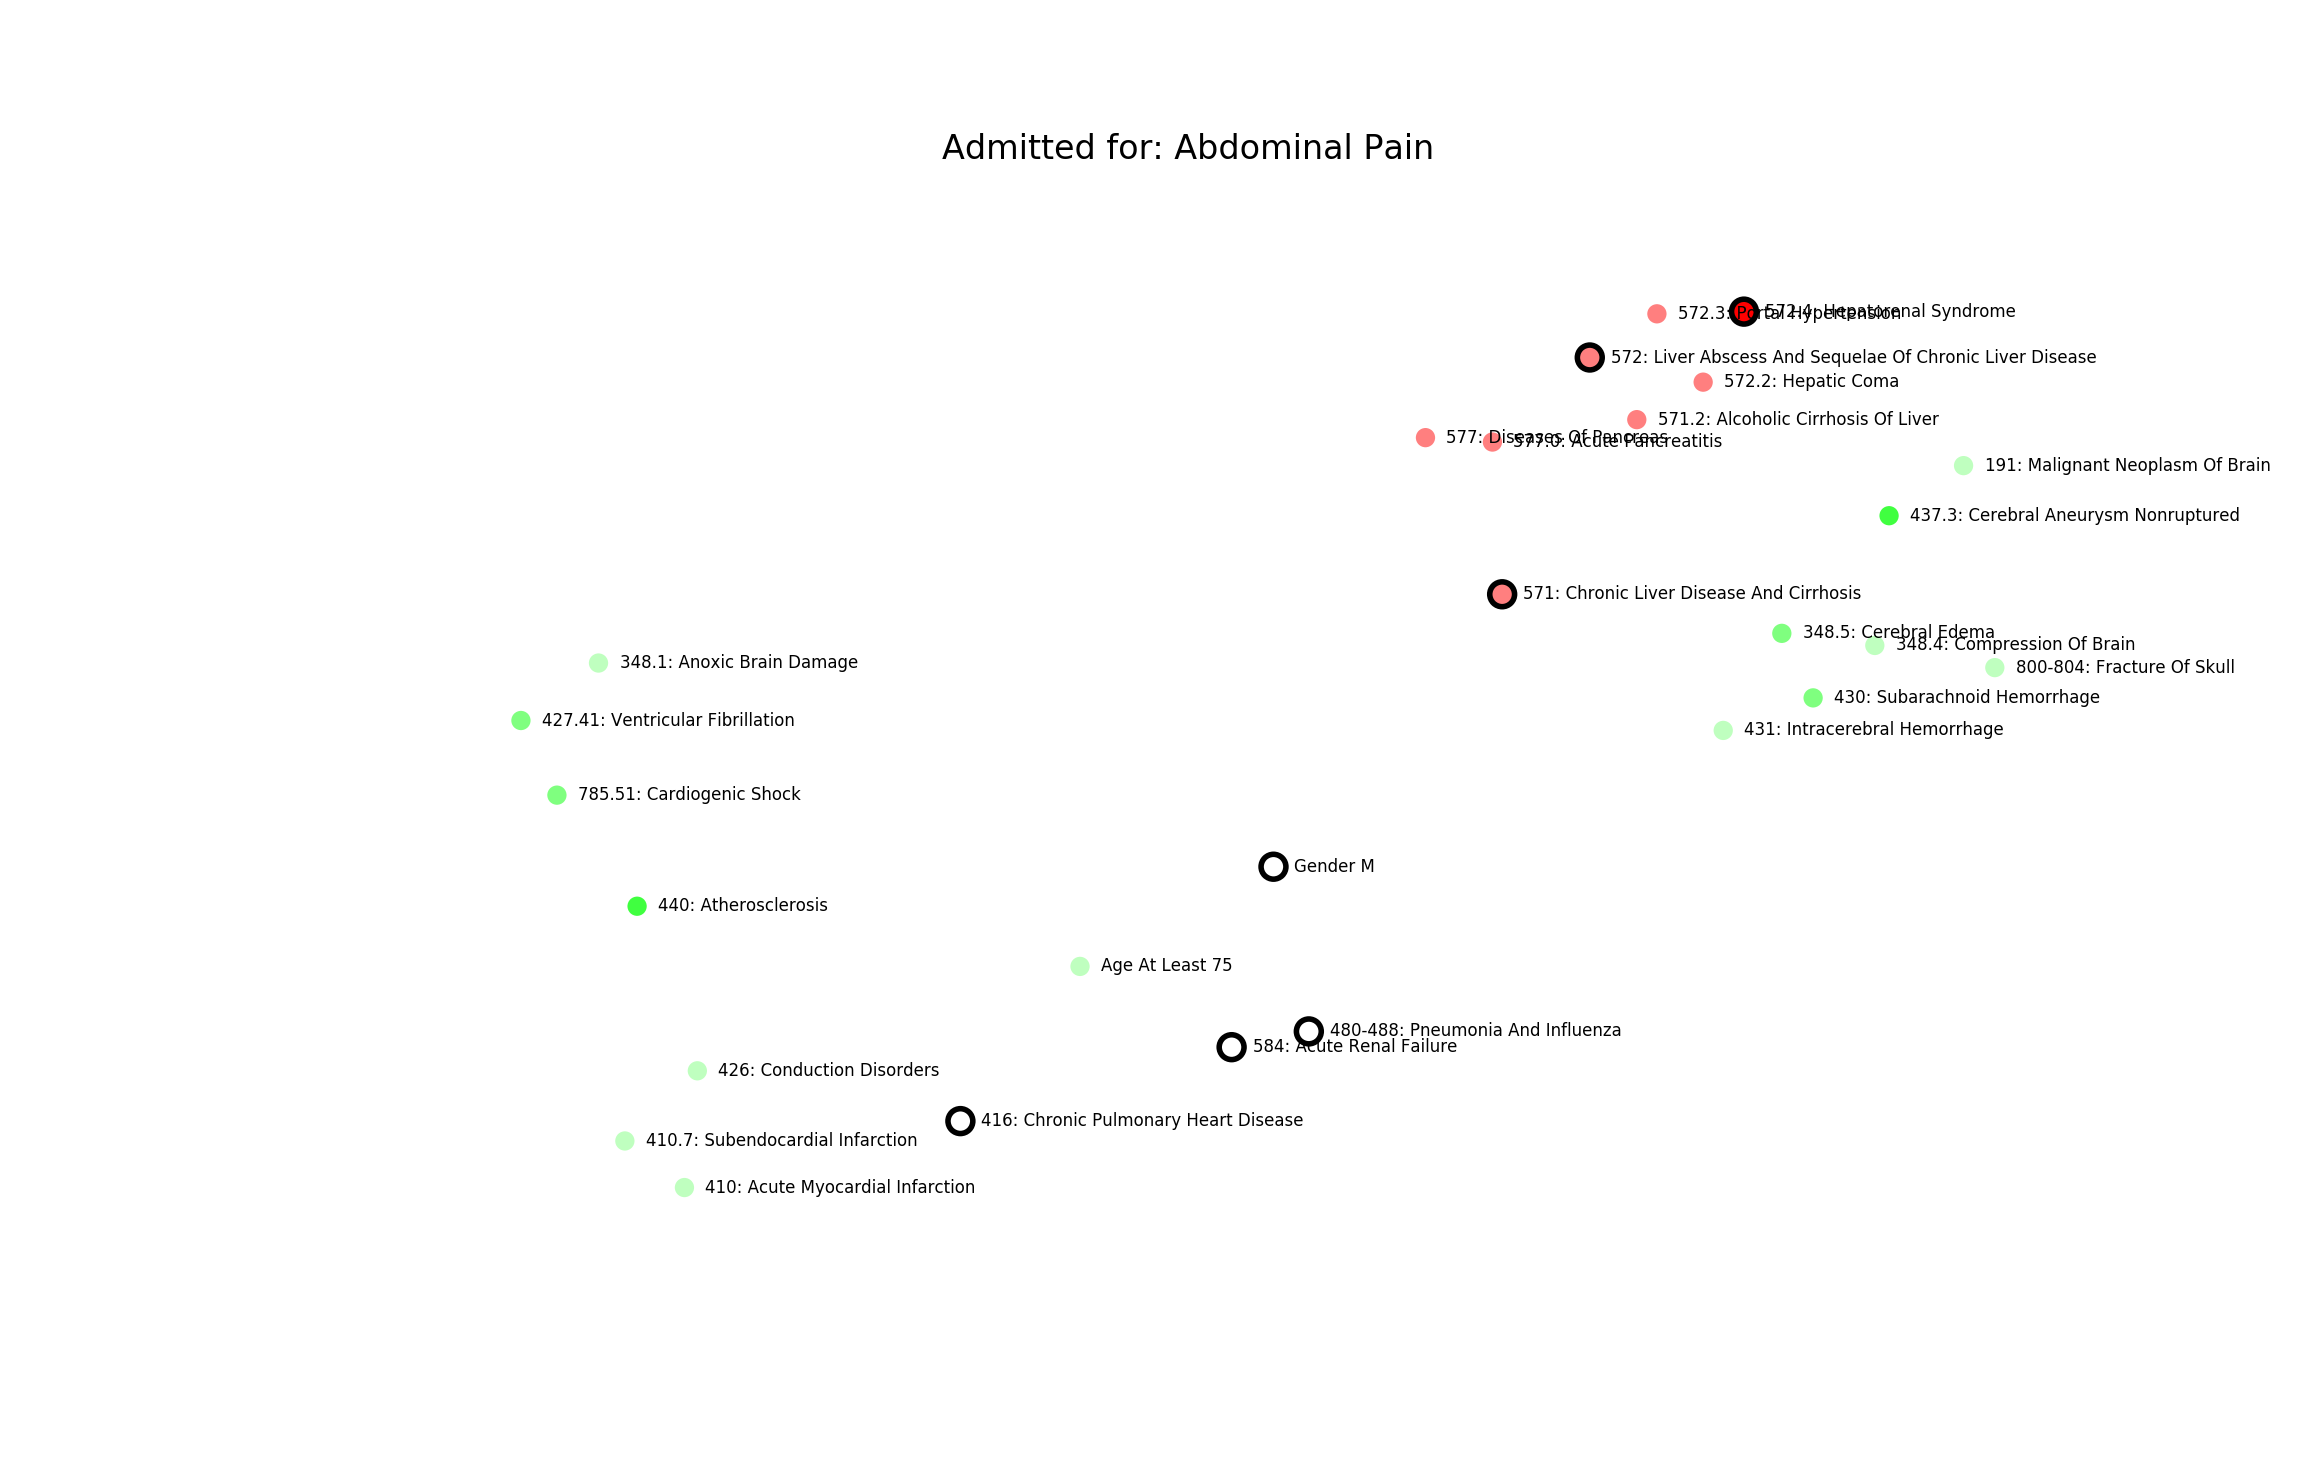
\includegraphics[width=\textwidth]{icu_map_liver}
\caption{Semantic Inference Abdominal Pain}
\vspace{12px}
This patient was admitted for ``Abdominal Pain".  The neural net predicted that they had low risk of brain and heart conditions (colored green).  It predicted high risk of liver conditions (colored red).  The patient was eventually diagnosed with chronic liver cirrhosis and a liver abscess among other things (circled in black).
\label{fig:icu_map_liver}
\end{figure}